\documentclass[a4paper, 12pt]{report}
\usepackage[top=2cm, bottom=2cm, left=2cm, right=2cm, centering, head=21.75 pt]{geometry}

\usepackage{amsmath}
\usepackage{amsthm}
\usepackage{subfigure}
\usepackage{booktabs}
\usepackage{caption}
\usepackage{amssymb}

\usepackage[italian]{babel}
\usepackage[utf8]{inputenc}
\usepackage{scrlayer-scrpage}
\ifoot[]{}
\cfoot[]{}
\ofoot[\pagemark]{\pagemark}
\pagestyle{scrplain}
\usepackage{mathptmx}
\usepackage{graphicx}
\usepackage{svg}
\usepackage{csquotes}
\usepackage[backend=biber, sorting=nty, ]{biblatex}
\appto{\bibsetup}{\raggedright}
\addbibresource{Thesis.bib}

\usepackage{titlesec}
\usepackage{float}

\usepackage{listings}
\renewcommand{\lstlistingname}{Code}
\usepackage{xcolor}
\definecolor{mygreen}{rgb}{0,0.6,0}
\definecolor{mygray}{rgb}{0.5,0.5,0.5}
\definecolor{mymauve}{rgb}{0.58,0,0.82}
\definecolor{darkgray}{rgb}{.4,.4,.4}
\definecolor{navy}{HTML}{000080}
\definecolor{purple}{rgb}{0.65, 0.12, 0.82}
\definecolor{codepurple}{rgb}{0.58,0,0.82}
\definecolor{backcolour}{rgb}{0.95,0.95,0.92}

\titleformat{\chapter}[block]
	{\normalfont\LARGE\bfseries}{\thechapter.}{0.5em}{\LARGE}
\titlespacing*{\chapter}{0pt}{-20pt}{25pt}

\usepackage{boxedminipage}
\usepackage{pgfplotstable}

\usepackage{times}

\begin{document}

	\tableofcontents
	\thispagestyle{empty}

	\listoffigures
	\thispagestyle{empty}
	\clearpage

	\chapter*{Abstract}
	\thispagestyle{empty}

		Il clustering non supervisionato non ha a disposizione una "ground
		truth" per valutare quanto il proprio operato sia effettivamente
		rappresentativo della struttura del dataset esaminato. Per adempiere
		a tale scopo sono state introdotte delle metriche in grado di stimare
		a posteriori (a clustering compiuto) le performance dell'algoritmo.
		Nel presente lavoro ne verrá presentata una in particolare, Silhouette.
		Verrà introdotta tale metrica, come calcolarla, alcune proprietà
		matematiche e verrá applicata al risultato del clustering su delle
		EHR (\textit{Electronic Health Records}). Verranno inoltre analizzati
		alcuni pacchetti per il linguaggio R che implementano Silhouette per
		determinare quale sia il migliore. Verranno infine fatte delle
		considerazioni in merito alla metrica stessa e alla sua capacitá
		di stimare le performance degli algoritmi di clustering.

	\chapter{Introduzione}
	\setcounter{page}{1}

		Con il termine \textbf{cluster analysis}, o semplicemente
		\textbf{clustering}, si intende \emph{''una tecnica di
		classificazione statistica atta a scoprire se gli individui
		di una popolazione ricadono all'interno di certi gruppi mediante
		comparazioni quantitative di loro molteplici caratteristiche``}
		\footnote{\texttt{https://www.merriam-webster.com/dictionary/cluster\%20analysis}}.
		Informalmente, il clustering consiste nel (tentare di) suddividere
		un insieme di dati in gruppi, chiamati appunto \textbf{cluster},
		di modo che ciascun gruppo contenga elementi simili fra di loro
		ma dissimili rispetto a quelli degli altri gruppi.

		La definizione del concetto di ``somiglianza'' sta nelle mani di
		chi compie il clustering. In genere, l'analisi dei dati si occupa
		di dati numerici (altezze, lunghezze, età, ampiezze), pertanto il
		modo più naturale per formalizzare la somiglianza è dato da una
		\textbf{funzione di distanza}. Matematicamente, una qualsiasi
		funzione $d: \mathbb{R} \times \mathbb{R} \rightarrow \mathbb{R}$
		è considerabile una funzione di distanza se possiede (almeno) le
		seguenti proprietà:

		\begin{itemize}
			\item
			Per ogni $x \in \mathbb{R}$, $d(x, x) = 0$;
			\item
			Per ogni $x, y \in \mathbb{R}$, se $x \neq y$ allora $d(x, y) > 0$;
			\item
			Per ogni $x, y \in \mathbb{R}$, $d(x, y) = d(y, x)$
			(\textbf{simmetria});
			\item
			Per ogni $x, y, z \in \mathbb{R}$, $d(x, z) \leq d(x, y) + d(y, z)$
			(\textbf{disuguaglianza triangolare}).
		\end{itemize}

		Un \textbf{algoritmo di clustering} non è altro che un algoritmo
		che abbia in input un insieme di dati e che abbia in output il
		risultato del clustering. Algoritmi di questo tipo fanno uso di
		una funzione di distanza per raggruppare gli elementi in cluster
		senza che sia necessario farlo manualmente.

		\begin{figure}[H]
			\centering
			\includesvg[width = 0.5\textwidth]{images/Cluster-2.svg}
			\caption{Ipotetico esempio di clustering}
		\end{figure}

		Gli algoritmi di clustering si dividono in due macrocategorie:
		\textbf{algoritmi supervisionati} e \textbf{algoritmi non
		supervisionati}. Nei primi, viene usato un insieme di dati per
		generalizzarne le proprietà, cercando di predire il risultato
		per dati futuri, mentre nei secondi si cerca di catturare le
		proprietà dei dati in sé e per sé.

		Una volta applicato un algoritmo di clustering su un certo insieme
		di dati, è ragionevole chiedersi se il risultato del clustering
		effettivamente rispecchi la struttura dei dati o se l'algoritmo
		abbia errato. Negli algoritmi di tipo supervisionato questo è
		semplice, perché è possibile comparare i dati ottenuti con il
		risultato atteso, similmente a come viene fatto in un modello di
		regressione.

		Negli algoritmi di tipo non supervisionato questo è molto
		più difficile, perché non c'è differenza fra l'insieme di
		dati utilizzato per costruire il modello e l'insieme di
		dati usato per testare il modello: sono lo stesso insieme.
		Una possibile soluzione al problema è data da delle statistiche,
		il cui valore rappresenta l'accuratezza del modello. Alcuni
		esempi sono: \textbf{Calinksi-Harabasz} \cite{Calinski01011974},
		\textbf{Davies-Bouldin} \cite{4766909} e \textbf{Dunn Index}
		\cite{Dunn01011974}.

		La statistica di interesse per questa tesi è Silhouette
		\cite{ROUSSEEUW198753}. Tale statistica, nelle parole
		dell'autore, si propone di rispondere alle seguenti domande:

		\begin{itemize}
			\item
			Il clustering è di buona qualità? In altre parole, gli elementi di
			uno stesso cluster sono fra di loro "vicini" ed al contempo "lontani"
			dagli elementi di tutti gli altri cluster?
			\item
			Quali sono gli elementi ben classificati, ovvero quelli che probabilmente
			si trovano nel cluster "giusto"?
			\item
			Quali sono gli elementi che è difficile stabilire con certezza in quali
			cluster vadano collocati, ovvero quelli che stanno "nel mezzo" fra più
			cluster?
			\item
			Il numero di cluster scelto è effettivamente rappresentativo del dataset
			o è 'artificioso'?
		\end{itemize}

		\begin{table}[h]
			\centering
			\footnotesize
			\begin{tabular}{| p{1.75cm} | p{1.75cm} | p{1.75cm} | p{1.75cm} | p{1.75cm} | p{1.75cm} |}
				\hline
				\multicolumn{6}{| p{12.5cm} |}{
					\textit{Identifying heterogeneous subgroups of systemic autoimmune
					diseases by applying a joint dimension reduction and clustering
					approach to immunomarkers} \cite{Chang2024}
				} \\
				\hline
				\textbf{Patologie} &
				\textbf{N. pazienti} &
				\textbf{Features} &
				\textbf{Algoritmi} &
				\textbf{Software} &
				\textbf{Metriche} \\
				\hline
				Lupus Eritematoso Sistemico, Artrite Reumatoide,
				Sindrome di Sjogren &
				11923 &
				biomarcatori (tradotti in variabili categoriali) &
				Multiple Correspondence Analysis K-means (clustering e dimensionality
				reduction insieme) &
				clustrd (R) &
				Silhouette \\
				\hline
				\multicolumn{6}{| p{12.5cm} |}{
					\textit{Association of comorbid-socioeconomic clusters with
					mortality in late onset epilepsy derived through unsupervised
					machine learning}
					\cite{Josephson_Gonzalez-Izquierdo_Engbers_Denaxas_Delgado-Garcia_Sajobi_Wang_Keezer_Wiebe_2023/10/01_2023}
				} \\
				\hline
				\textbf{Patologie} &
				\textbf{N. pazienti} &
				\textbf{Features} &
				\textbf{Algoritmi} &
				\textbf{Software} &
				\textbf{Metriche} \\
				\hline
				Epilessia (tardiva) &
				11307 &
				Fattori di rischio, comorbiditá (indice di Charlson) &
				Agglomerative Hierarchical Clustering &
				scikit-learn (Python), Python 3.6.3, Stata 16.1 &
				Silhouette, Davies-Bouldin \\
				\hline
				\multicolumn{6}{| p{12.5cm} |}{
					\textit{Exploration of critical care data by using unsupervised
					machine learning} \cite{HYUN2020105507}
				} \\
				\hline
				\textbf{Patologie} &
				\textbf{N. pazienti} &
				\textbf{Features} &
				\textbf{Algoritmi} &
				\textbf{Software} &
				\textbf{Metriche} \\
				\hline
				&
				1503 &
				Valori di test di routine di laboratorio (BUN, creatinina, glucosio, ...) &
				Kmeans &
				R 3.5.2 &
				Total within-cluster variation, Silhouette, Gap statistic \\
				\hline
				\multicolumn{6}{| p{12.5cm} |}{
					\textit{Identifying and evaluating clinical subtypes of Alzheimer’s
					disease in care electronic health records using unsupervised machine
					learning} \cite{Alexander2021}
				} \\
				\hline
				\textbf{Patologie} &
				\textbf{N. pazienti} &
				\textbf{Features} &
				\textbf{Algoritmi} &
				\textbf{Software} &
				\textbf{Metriche} \\
				\hline
				Malattia di Alzheimer &
				10065 &
				sintomi tipici, comorbiditá, dati demografici &
				K-Means, Kernel K-means, Affinity Propagation, Latent Class Analysis &
				&
				Silhouette, Coefficiente di Jaccard \\
				\hline
				\multicolumn{6}{| p{12.5cm} |}{
					\textit{Utilization of Deep Learning for Subphenotype Identification
					in Sepsis-Associated Acute Kidney Injury} \cite{01277230-202011000-00006}
				} \\
				\hline
				\textbf{Patologie} &
				\textbf{N. pazienti} &
				\textbf{Features} &
				\textbf{Algoritmi} &
				\textbf{Software} &
				\textbf{Metriche} \\
				\hline
				Sepsi &
				4001 &
				Segni vitali, test di laboratorio &
				K-Means &
				scikit-learn (Python), matplotlib (Python), SAS 9.4, R 3.4.3 &
				Silhouette, Davies-Bouldin, Calinksi-Harabasz \\
				\hline
			\end{tabular}
			\caption{Riassunto degli articoli scientifici che applicano Silhouette su EHR}
			\label{tbl:ehr}
		\end{table}

		\begin{table}[h]
			\centering
			\footnotesize
			\begin{tabular}{| p{3.25cm} | p{1.75cm} | p{2.5cm} | p{1.5cm} | p{1.5cm} |}
				\hline
				\multicolumn{5}{| p{12.5cm} |}{
					\textit{Silhouette Index as clustering evaluation tool}
					\cite{10.1007/978-3-030-52348-0_2}
				} \\
				\hline
				\textbf{Sintesi} &
				\textbf{Algoritmi} &
				\textbf{Dataset} &
				\textbf{Software} &
				\textbf{Metriche} \\
				\hline
				È possibile utilizzare Silhouette come "stopping rule" direttamente
				all'interno di un algoritmo di clustering? &
				RPCT &
				Dataset artificiale, generato mediante \texttt{cluster.Gen}, FCPS
				Dataset artificiale costituito da tre distribuzioni uniformi &
				clusterSim (R) &
				Adjusted Rand Index \\
				\hline
				\multicolumn{5}{| p{12.5cm} |}{
					\textit{Performance evaluation of the Silhouette index}
					\cite{10.1007/978-3-319-19369-4_5}
				} \\
				\hline
				\textbf{Sintesi} &
				\textbf{Algoritmi} &
				\textbf{Dataset} &
				\textbf{Software} &
				\textbf{Metriche} \\
				\hline
				Qual'è il modo corretto per calcolare la Silhouette media? &
				Complete-linkage, single-linkage &
				Quattro dataset artificiali con una struttura di cluster ben definita,
				\texttt{Iris}, \texttt{Wine} &
				&
				\\
				\hline
				\multicolumn{5}{| p{12.5cm} |}{
					\textit{A comparison of clustering quality indices using outliers and noise}
					\cite{doi:10.3233/IDA-2012-0545}
				} \\
				\hline
				\textbf{Sintesi} &
				\textbf{Algoritmi} &
				\textbf{Dataset} &
				\textbf{Software} &
				\textbf{Metriche} \\
				\hline
				Quali sono le prestazioni di Silhouette rispetto ad altre metriche? &
				K-means, model-based clustering, hierarchical clustering, algoritmo "random" &
				\texttt{clear} (struttura di cluster è ben definita),
				\texttt{out} (parte dei dati sono noise),
				\texttt{noi} (parte delle dimensioni sono noise) &
				&
				Calinski-Harabasz, C-index, Davies-Bouldin, Gamma, ARI \\
				\hline
				\multicolumn{5}{| p{12.5cm} |}{
					\textit{Condensed Silhouette: An Optimized Filtering Process for Cluster Selection in K-Means}
					\cite{NAGHIZADEH2020205}
				} \\
				\hline
				\textbf{Sintesi} &
				\textbf{Algoritmi} &
				\textbf{Dataset} &
				\textbf{Software} &
				\textbf{Metriche} \\
				\hline
				Nel caso di algoritmi di clustering partizionale, è possibile
				semplificare ulteriormente Silhouette? &
				K-Means &
				7 microarray gene expressions (migliaia di features), 7
				dataset reali famosi (come Iris) &
				Scikit-Learn (Python) &
				\\
				\hline
				\multicolumn{5}{| p{12.5cm} |}{
					\textit{CUBOS: An Internal Cluster Validity Index for Categorical Data}
					\cite{Gao2019CUBOSAI}
				} \\
				\hline
				\textbf{Sintesi} &
				\textbf{Algoritmi} &
				\textbf{Dataset} &
				\textbf{Software} &
				\textbf{Metriche} \\
				\hline
				È possibile estendere Silhouette per utilizzarla su valori discreti? &
				IDC &
				K-Modes &
				UCI &
				\\
				\hline
			\end{tabular}
			\caption{Riassunto degli articoli scientifici che studiano Silhouette da un punto di vista teorico}
			\label{tbl:theory}
		\end{table}

	\chapter{Metodi e strumenti utilizzati}

		\section{Dataset}

			Per quanto riguarda l'applicare algoritmi di clustering a
			dataset reali, come dataset ho utilizzato delle cartelle
			cliniche elettroniche (EHR). Questi dataset, in formato
			\texttt{.csv} (\emph{comma separated value}), sono liberamente
			utilizzabili. Per comodità, ho indicato tali dataset con la
			malattia a cui si riferiscono: \texttt{Diabetes},
			\texttt{Neuroblastoma}, \texttt{CardiacArrest},
			\texttt{HeartFailure}, \texttt{Sepsis}. Nell'intestazione
			dei plot è comunque possibile leggere il nome completo
			del rispettivo dataset.

			Per quanto riguarda la valutazione delle performance delle
			implementazioni di Silhouette ho utilizzato due dataset da
			me generati, indicati con \texttt{sc\_dataset\_good} e
			\texttt{sc\_dataset\_bad}. Li ho costruiti utilizzando la
			funzione \texttt{rnorm}, che genera dei punti casuali a
			partire da una distribuzione normale bivariata. Dataset
			simili compaiono anche nella descrizione della Silhouette.

			\texttt{sc\_dataset\_good} è costituito da due distribuzioni
			normali fuse insieme, entrambe con una deviazione standard
			molto bassa, di modo che i punti siano concentrati attorno
			alla media. \texttt{sc\_dataset\_bad} è costituito da una
			sola distribuzione normale bivariata centrata in $(0, 0)$ e
			con una deviazione standard molto ampia, di modo che i punti
			siano molto dispersi. I loro scatter plot sono riportati in
			Figura~\ref{fig:sc1} e Figura~\ref{fig:sc2} rispettivamente.

			\begin{figure}[H]
				\centering
				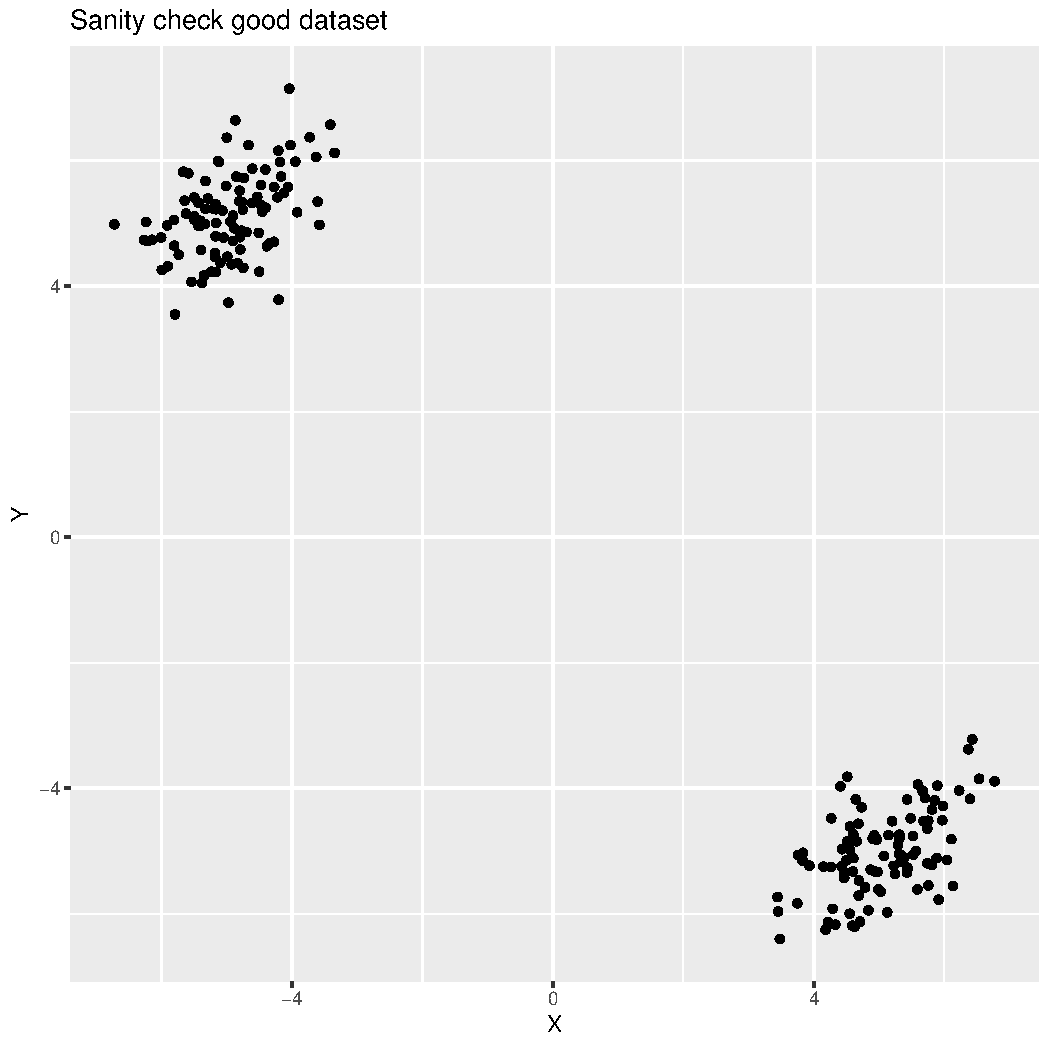
\includegraphics[width = 0.75\textwidth, height = 0.45\textheight]{doc/sc_dataset_good.pdf}
				\caption{Scatter plot di \texttt{sc\_dataset\_good}.
				Si noti la struttura di cluster ben definita.}
				\label{fig:sc1}
			\end{figure}

			\begin{figure}[H]
				\centering
				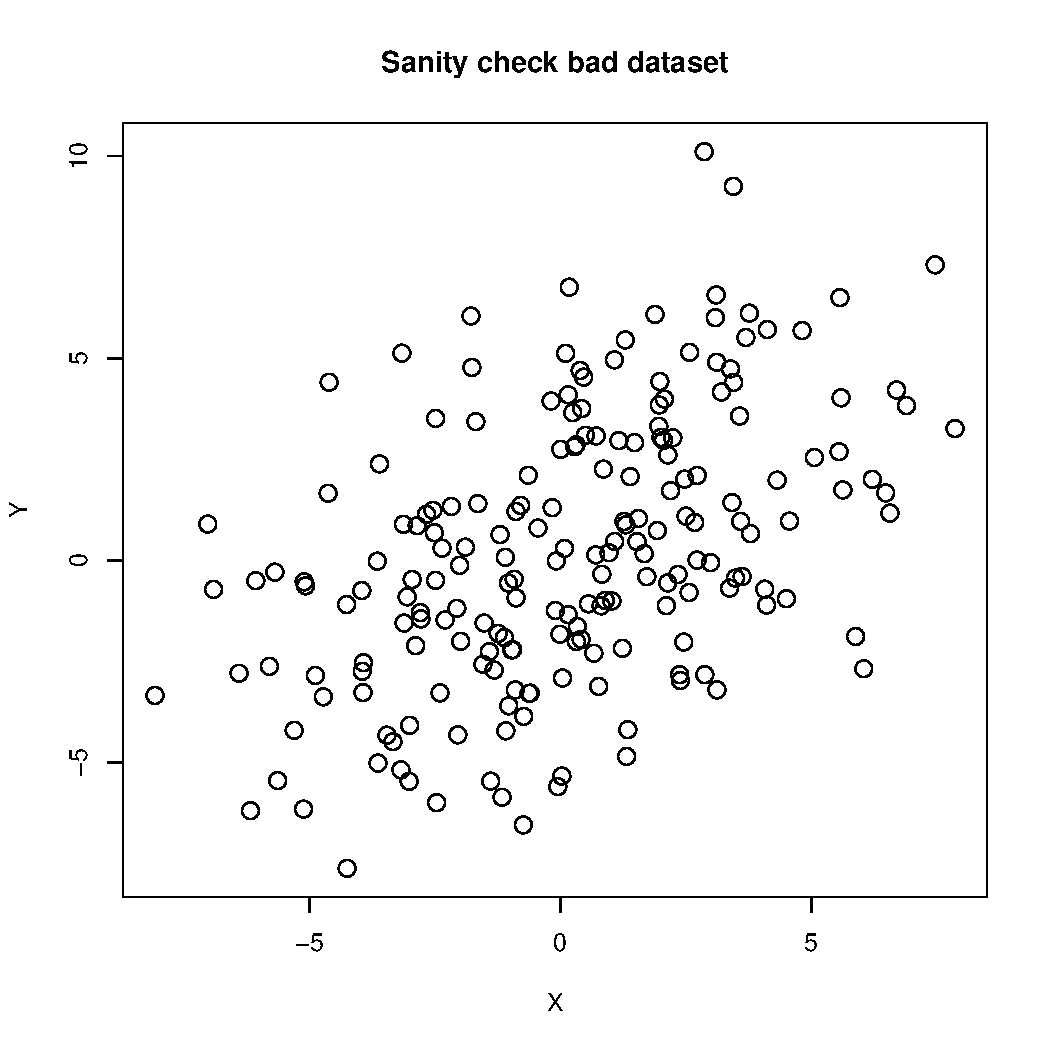
\includegraphics[width = 0.75\textwidth, height = 0.45\textheight]{doc/sc_dataset_bad.pdf}
				\caption{Scatter plot di \texttt{sc\_dataset\_bad}.
				Si noti l'assenza della struttura di cluster.}
				\label{fig:sc2}
			\end{figure}

			Infine, diversi esempi si rifanno ad un dataset molto famoso
			chiamato \texttt{iris} \cite{https://doi.org/10.1111/j.1469-1809.1936.tb02137.x}.
			Tale dataset è costituito da $150$ elementi estratti da una
			popolazione di fiori, ciascuno contenente cinque attributi,
			in ordine: lunghezza del sepalo (in centimetri), larghezza
			del sepalo, lunghezza del petalo, larghezza del petalo e
			specie del fiore (\emph{Iris setosa}, \emph{Iris virginica}
			oppure \emph{Iris versicolor}). Dato che l'ultimo attributo
			non è numerico, viene in genere scartato. Nella
			Tabella~\ref{tab:iris-sample} sono riportati alcuni
			elementi di tale dataset.

			\begin{table}[H]
				\centering
				\begin{tabular}{c c c c c}
					\hline
					\textbf{Sepal.Length} &
					\textbf{Sepal.Width} &
					\textbf{Petal.Length} &
					\textbf{Petal.Width} &
					\textbf{Species} \\
					\hline
					5.1 & 3.5 & 1.4 & 0.2 & setosa \\
					4.9 & 3.0 & 1.4 & 0.2 & setosa \\
					4.7 & 3.2 & 1.3 & 0.2 & setosa \\
					4.6 & 3.1 & 1.5 & 0.2 & setosa \\
					5.0 & 3.6 & 1.4 & 0.2 & setosa \\
					5.4 & 3.9 & 1.7 & 0.4 & setosa \\
					4.6 & 3.4 & 1.4 & 0.3 & setosa \\
					\hline
				\end{tabular}
				\caption{Primi elementi del dataset \texttt{iris},
				così come compare nel linguaggio \texttt{R}.}
				\label{tab:iris-sample}
			\end{table}

		\section{Funzioni di distanza}

			Si supponga di avere a disposizione un dataset di dimensione
			$N \times M$, dove $N$ indica il numero degli elementi e $M$ è
			il numero di attributi. Si assuma, per semplicità, che tutti
			gli attributi siano tutti dati numerici (altezze, lunghezze,
			capacità, ecc...) e che ogni valore di ogni attributo sia noto.

			Per ciascuna coppia di elementi $i$ e $j$ del dataset è possibile
			calcolare la loro distanza mediante una funzione di distanza. La
			funzione di distanza più intuitiva è la \textbf{distanza Euclidea},
			che equivale alla distanza fra due punti nel piano cartesiano
			$n$-dimensionale, definita come segue:

			\begin{equation}
				d(i, j) =
				\sqrt{\sum_{m = 1}^{M} (f_{i, m} - f_{j, m})^{2}} =
				\sqrt{(f_{i, 1} - f_{j, 1})^{2} + \dots +
					(f_{i, M} - f_{j, M})^{2}}
			\end{equation}

			Dove $f_{i, m}$ e $f_{j, m}$ indicano il valore del $m$-esimo
			attributo per, rispettivamente, l'$i$-esimo ed il $j$-esimo
			elemento del dataset.

			Un'altro esempio di distanza è la \textbf{distanza di Manhattan},
			calcolata come la somma fra le differenze in modulo di ciascuna
			coppia di attributi:

			\begin{equation}
				d(i, j) =
				\sum_{m = 1}^{M} |f_{i, m} - f_{j, m}| =
				|f_{i, 1} - f_{j, 1}| + \dots +
				|f_{i, M} - f_{j, M}|
			\end{equation}

			Ultimo esempio di distanza è la \textbf{distanza di Jaccard},
			calcolata a partire dal numero di elementi che due insiemi $A$
			e $B$ hanno in comune ed al numero di elementi che non hanno
			in comune:

			\begin{equation}
				d(A, B) = 1 - \frac{|A \cap B|}{|A \cup B|}
			\end{equation}

			A partire da un dataset di $N$ elementi e da una funzione
			di distanza è possibile costruire quella che viene chiamata
			\textbf{matrice delle distanze}. Tale matrice ha dimensione
			$N \times N$ e, in ciascuna cella $(i, j)$, è presente la
			distanza $d(i, j)$ fra i due elementi. La Tabella~\ref{tab:dist}
			contiene un esempio di matrice delle distanze.

			\begin{table}[h]
				\begin{equation*}
					\begin{bmatrix}
						0.5385165 & & & & & & \\
						0.5099020 & 0.3000000 & & & & & \\
						0.6480741 & 0.3316625 & 0.2449490 & & & & \\
						0.1414214 & 0.6082763 & 0.5099020 & 0.6480741 & & & \\
						0.6164414 & 1.0908712 & 1.0862780 & 1.1661904 & 0.6164414 & & \\ 
						0.5196152 & 0.5099020 & 0.2645751 & 0.3316625 & 0.4582576 & 0.9949874 & \\ 
						0.1732051 & 0.4242641 & 0.4123106 & 0.5000000 & 0.2236068 & 0.7000000 & 0.4242641 \\
					\end{bmatrix}
				\end{equation*}

				\caption{Matrice delle distanze per il dataset \texttt{iris},
				scartando l'ultimo attributo in quanto non numerico, usando
				come funzione di distanza la distanza Euclidea. Per questioni
				di spazio sono presenti solamente i primi 7 elementi. Si noti
				come la matrice sia riportata solo per metà, perché per
				definizione una matrice delle distanze è sempre simmetrica.}
				\label{tab:dist}
			\end{table}

			La distanza Euclidea è la funzione di distanza che viene
			utilizzata di default nella maggior parte delle implementazioni
			di default degli algoritmi di clustering. Inoltre, nella maggior
			parte dei casi, un algoritmo di clustering non necessita di
			utilizzare una funzione di distanza specifica. Pertanto, se non
			specificato diversamente, quando ci si riferisce ad una funzione
			di distanza generica si intende la distanza Euclidea.

		\section{Algoritmi di clustering}

			Gli algoritmi di clustering sono innumerevoli, ed è
			impossibile testarli tutti. In questa tesi ne ho scelti
			quattro: \textbf{K-Means} \cite{1056489} e la sua variante
			\textbf{K-Medians}, \textbf{DBSCAN} \cite{10.5555/3001460.3001507}
			e \textbf{HDBSCAN} \cite{10.1007/978-3-642-37456-2_14}.

			\subsection{Clustering partizionale: K-Means e K-Medians}

				\textbf{K-Means} e \textbf{K-Medians} sono esempi di algoritmi
				di clustering \textbf{partizionale}, ovvero che suddividono
				l'insieme di dati in un certo numero di cluster operando diversi
				"raffinamenti" spostando uno o più elementi da un cluster all'altro
				fino a raggiungere la precisione desiderata. L'algoritmo può essere
				descritto come segue:

				\begin{enumerate}
					\item
						Sia scelga un intero $k$. Tale valore sarà il numero di cluster;
					\item
						Si scelgano $k$ elementi qualsiasi del dataset, detti \textbf{seed}.
						Tali seed fungeranno da \textbf{centroidi} iniziali, ovvero da elementi
						che rappresentano il "baricentro" o il "punto medio" di ciascun cluster;
					\item
						Per ciascun elemento del dataset che non è un centroide, si calcoli
						la distanza fra tale elemento e tutti i centroidi. L'elemento viene
						assegnato alla partizione il cui centroide ha la più piccola distanza
						da questo;
					\item
						Per ogni cluster se ne ricalcolino i centroidi, operando la media
						aritmetica dei suoi valori;
					\item
						Se è stato raggiunto un criterio di terminazione, l'algoritmo termina.
						Altrimenti, si riprende dal punto 3.
				\end{enumerate}

				Si noti come l'algoritmo non specifichi un criterio di terminazione. Un criterio
				molto semplice consiste nel fissare un $\epsilon$ e valutare di quanto
				si discosta il nuovo valore dei centroidi (calcolato al punto 4) dal
				valore precedente: se questo scostamento è inferiore ad $\epsilon$,
				l'algoritmo termina. Un criterio simile prevede di fissare un $\epsilon$
				e di terminare l'algoritmo se il numero di elementi che vengono assegnati
				ad un cluster diverso alla fine della corrente iterazione è inferiore ad
				$\epsilon$.

				\begin{figure}[H]
					\centering
					\includesvg{images/K-Means-Example}
					\caption{Applicazione dell'algoritmo K-Means ad un ipotetico dataset;
					i tre colori indicano i tre cluster individuati dall'algoritmo (By I,
					Weston.pace, CC BY-SA 3.0, https://commons.wikimedia.org/w/index.php?curid=2463085).}
					\label{fig:k-means-example}
				\end{figure}

				L'algoritmo K-Medians è una variante di K-Means che usa le mediane dei
				cluster come centroidi anziché le loro medie. Per tal motivo, mentre
				K-Means può utilizzare sostanzialmente qualsiasi funzione di distanza,
				K-Medians utilizza sempre la distanza di Manhattan.

				Sebbene K-Means e K-Medians siano efficienti (se il numero di
				iterazioni è piccolo, il tempo di esecuzione è quasi-lineare) e
				anche estremamente semplici, tanto da comparire come subroutine
				in algoritmi più complessi, presentano dei problemi. Ad esempio,
				dato che ogni elemento ha lo stesso peso nel computo dei centroidi,
				anche un solo elemento che abbia valori anomali può destabilizzare
				completamente il risultato finale. Inoltre, il parametro $k$ che
				determina il numero di cluster potrebbe non avere alcuna relazione
				con l'effettivo numero di cluster (se esistono) nell'insieme di
				dati, e quindi un valore scorretto di $k$ porta a risultati che
				non rispecchiano per nulla la vera struttura di cluster. Infine,
				il raggruppamento di più elementi sulla base di una distanza genera
				dei cluster di forma ellittica, ma non tutti i dataset hanno una
				struttura di cluster con questa forma.

			\subsection{Clustering per densità: DBSCAN}

				\textbf{DBSCAN} è un esempio di algoritmo di clustering \textbf{per
				densità}, ovvero che costruisce i cluster a partire da come gli
				elementi di un dataset sono aggregati. In questo senso, i cluster
				figurano come regioni di spazio densamente popolate, di forma del
				tutto arbitraria, separate da spazio poco popolato.

				DBSCAN prevede che vengano innanzitutto scelti due valori, un intero
				chiamato MinPts ed un numero reale positivo $\epsilon$. A partire da
				questi, per ogni elemento $p$ del dataset è possibile definire un
				insieme $N_{\epsilon}(p)$, chiamato $\epsilon$\textbf{-vicinato}
				($\epsilon$\textbf{-neighbourhood}). Tale insieme contiene tutti i
				punti $q$ che hanno distanza da $p$ inferiore a $\epsilon$:

				\begin{equation*}
					N_{\epsilon} (p) = \{q | d(p, q) \leq \epsilon\}
				\end{equation*}

				Ogni elemento $p$ del dataset viene classificato sulla base del numero
				di elementi di $N_{\epsilon}(p)$:

				\begin{itemize}
					\item
					Se $N_{\epsilon}(p)$ ha almeno MinPts elementi, si dice che $p$ è un
					\textbf{core point};
					\item
					Se $N_{\epsilon}(p)$ ha meno di MinPts elementi ma $p$ si trova
					nell'$\epsilon$-vicinato di un altro elemento, allora si dice che
					$p$ è un \textbf{border point};
					\item
					Se un elemento non non è né un core point né un border
					point, è detto \textbf{noise point}.
				\end{itemize}

				Si dice che un elemento $q$ è \textbf{direttamente raggiungibile}
				da $p$ se $p$ è un core point e $q$ si trova nell'$\epsilon$-vicinato
				di $p$. Se un elemento $r$ è direttamente raggiungibile da $q$ e $q$
				è direttamente raggiungibile da un elemento $p$, allora si dice che
				$r$ è \textbf{indirettamente raggiungibile} da $p$ (si noti come
				la raggiungibilità non sia una proprietà necessariamente simmetrica).

				\begin{figure}[H]
					\centering
					\includesvg[width = 0.5\textwidth]{images/DBSCAN-Illustration.svg}
					\caption{Ipotetica classificazione di alcuni elementi, usando
					MinPts = 4. Gli elementi in rosso sono dei core point, perché
					hanno 4 o più elementi nel loro $\epsilon$-vicinato. Gli elementi
					in giallo sono invece border point, perché hanno meno di 4 elementi
					nel loro $\epsilon$-vicinato ma sono nell'$\epsilon$-vicinato di
					almeno un core point. Infine, gli elementi in blu sono dei
					noise point, perché oltre ad avere meno di 4 elementi nel loro
					$\epsilon$-vicinato non sono nell'$epsilon$-vicinato di alcun
					core point (By Chire - Own work, CC BY-SA 3.0,
					https://commons.wikimedia.org/w/index.php?curid=17045963).}
					\label{fig:dbscan-illustration}
				\end{figure}

				Quando DBSCAN viene invocato viene inizializzato un cluster
				$C$, dopodiché viene costruito l'$\epsilon$-vicinato di ogni
				elemento $p$ che non sia stato ancora ispezionato. Se tale
				insieme ha meno di MinPts elementi, allora $p$ è certamente
				un noise point: questo perché è troppo isolato per poter
				essere un core point e, non essendo ancora stato ispezionato,
				non può trovarsi nell'$\epsilon$-vicinato di nessun altro punto.

				Se invece l'$\epsilon$-vicinato di $p$ ha almeno MinPts
				elementi, allora tale elemento è certamente un core point.
				Viene allora costruito un cluster $C$ nel quale $p$ viene
				inserito, dopodiché vengono osservati tutti gli elementi
				$q$ che si trovano nell'$\epsilon$-vicinato di $p$.
				Se $q$ non è mai stato ispezionato, si osserva
				l'$\epsilon$-vicinato di $q$ a sua volta: se questo
				contiene più elementi dell'$\epsilon$-vicinato di $p$,
				allora $N_{\epsilon}(q)$ e $N_{\epsilon}(p)$ vengono
				uniti in un insieme unico, perché gli elementi
				dell'$\epsilon$-vicinato di $q$ sono indirettamente
				raggiungibili a partire da $p$. Se $q$ non appartiene
				ad alcun cluster, allora viene aggiunto al cluster in esame.

				\begin{figure}[H]
					\centering
					\includesvg[width = 0.5\textwidth]{images/DBSCAN-density-data.svg}
					\caption{Risultato dell'applicazione dell'algoritmo DBSCAN su un
					ipotetico dataset. Le aree in blu e in verde rappresentano i due
					cluster, mentre i punti in grigio sono i noise point (By Chire -
					Own work, CC BY-SA 3.0, https://commons.wikimedia.org/w/index.php?curid=17085332)}
					\label{fig:dbscan-density-data}
				\end{figure}

				Si osservi come la scelta di $\epsilon$ e MinPts influisca di molto
				sul risultato finale. Infatti, scegliendo un valore di $\epsilon$ o
				di MinPts troppo piccolo, quasi tutti gli elementi verranno classificati
				come noise point, e quindi quasi tutti scartati. D'altro canto, un valore
				di $\epsilon$ o di MinPts troppo grande potrebbe indurre un clustering
				dove quasi tutti i punti sono inclusi nello stesso cluster.

				A differenza di K-Means e K-Medians, che costruiscono sempre cluster
				di forma ellissoidale, DBSCAN costruisce cluster di qualsiasi forma.
				Questo è sia un aspetto positivo, perché in questo modo è possibile
				catturare strutture di cluster molto più variegate, sia negativo,
				perché la densità di un'area non sottende necessariamente alla
				presenza di un cluster, e non tutte le aree dense lo sono allo
				stesso modo. Occorre però evidenziare come, nonostante sia leggermente
				inferiore a K-Means e K-Medians in termini di tempo di esecuzione
				($O n \log(n)$, con $n$ numero di elementi del dataset), le sue
				prestazioni sono state empiricamente dimostrate come molto competitive.

			\subsection{Clustering gerarchico: HDBSCAN}

				\textbf{HDBSCAN} è un esempio di algoritmo di clustering
				\textbf{gerarchico}, ovvero che costruisce i cluster formando
				una struttura ad albero \footnote{In realtà, HDBSCAN è un
				algoritmo ibrido fra il paradigma per densità ed il paradigma
				gerarchico. Un esempio semplice di algoritmo di clustering
				``puramente'' gerarchico é \textbf{UPGMA} \cite{Sokal1958ASM}.}

			Per K-Means, è stato testato un numero di cluster compreso fra $2$ e
			$6$, mentre per K-Medians fra $2$ e $10$.

			Per DBSCAN e HDBSCAN, MinPts è stato scelto nel range dal numero delle
			dimensioni del dataset al doppio più uno delle dimensioni del dataset.

			Per DBSCAN, $\epsilon$ è stato scelto partizionando la distanza massima
			in parti uguali.

		\section{Calcolo di Silhouette}

			Per poter calcolare Silhouette è prima necessario introdurre due
			quantità assegnate a ciascun elemento $i$ del dataset, indicate
			rispettivamente con $a(i)$ e $b(i)$. A partire da queste sará
			possibile calcolare un valore $s(i)$, e la media di tutti gli
			$s(i)$ per ciascun $i$ sará il valore di interesse.

			Dato un dataset con $N$ elementi e $D$ dimensioni, se ne calcoli
			la matrice delle distanze e si applichi su questo un algoritmo
			di clustering. Si supponga che tale algoritmo individui $K$
			cluster; per ciascuno di questi, è interamente noto sia il
			numero di suoi elementi sia a quale cluster ciascun elemento
			del dataset è stato assegnato.

			Preso un elemento $i$ del dataset, sia $A$ il cluster in cui l'algoritmo
			lo ha riposto. Ammesso che $A$ contenga altri elementi all'infuori di $i$,
			è possibile definire $a(i)$ come distanza media fra $i$ e tutti gli elementi
			di $A$ escluso $i$ stesso:

			\begin{equation}
				a(i) = \frac{1}{|A| - 1} \sum_{j \in \{A - \{i\}\}} d(i, j)
			\end{equation}

			Tale valore misura quanto un cluster è \textit{coeso}, nel senso
			che se tale valore è piccolo per tutti gli elementi del cluster,
			questi si trovano fra loro vicini. Per tale motivo, $a(i)$ viene
			anche chiamata \textbf{distanza intra-cluster}.

			Dopodiché, in maniera simile, per un cluster $C$ diverso da $A$
			è possibile definire $D(i, C)$ come la distanza media fra $i$
			(che appartiene ad $A$) e gli elementi di $C$:

			\begin{equation*}
				D(i, C) = \frac{1}{|C|} \sum_{j \in C} d(i, j)
			\end{equation*}

			Tale valore misura quanto un cluster è \textit{separato}, nel senso
			che se tale valore è grande per tutti gli elementi del cluster a cui
			$i$ appartiene, il cluster nel suo complesso si trova molto distante
			da tutti gli altri. Per tale motivo $D(i, C)$ viene anche chiamata
			\textbf{distanza inter-cluster}.

			Assumendo che il numero di cluster sia più di uno, per uno stesso elemento
			$i$ è possibile calcolare la distanza inter-cluster per ogni possibile
			cluster $C$ distinto da $A$. Fra questi $K - 1$ cluster, è di particolare
			interesse il cluster che ha il più piccolo valore di distanza inter-cluster
			per $i$, chiamato \textbf{neighboring cluster}. Questo perché tale cluster
			è quello che, se il cluster $A$ non esistesse, sarebbe la miglior scelta
			per catalogare $i$, essendo quello con gli elementi più vicini ad $i$.

			Se il neighboring cluster per $i$ è il cluster $C'$, la distanza
			inter-cluster $D(i, C')$ viene indicata con $b(i)$:

			\begin{equation}
				b(i) = min_{C \neq A} D(i, C)
			\end{equation}

			Una volta calcolato $a(i)$ e $b(i)$ per l'elemento $i$ del dataset, è
			possibile assegnarvi un valore di Silhouette $s(i)$, così calcolato:

			\begin{equation}
				s(i) = \frac{b(i) - a(i)}{max\{a(i), b(i)\}}
			\end{equation}

			Se l'elemento $i$ si trova in un cluster che contiene solamente sé stesso,
			per convenzione il valore $s(i)$ viene posto a $0$ (è una scelta arbitraria,
			ma è anche quella più neutra).

			È facile verificare che, per qualsiasi elemento $i$:

			\begin{equation*}
				-1 \leq s(i) \leq 1
			\end{equation*}

			Si assuma infatti che $b(i) \geq a(i)$. L'espressione diventa:

			\begin{equation*}
				s(i) = \frac{b(i) - a(i)}{b(i)} =
				\frac{b(i)}{b(i)} - \frac{a(i)}{b(i)} =
				- \frac{a(i)}{b(i)}
			\end{equation*}

			Avendo assunto che $b(i)$ sia maggiore di $a(i)$, tale frazione è una
			frazione propria, e pertanto il suo valore è racchiuso nell'intervallo
			$[-1, 0]$.

			Si assuma invece $a(i) > b(i)$. L'espressione diventa:

			\begin{equation*}
				s(i) = \frac{b(i) - a(i)}{a(i)} =
				\frac{b(i)}{a(i)} - \frac{a(i)}{a(i)} =
				\frac{b(i)}{a(i)}
			\end{equation*}

			Avendo assunto che $a(i)$ sia maggiore di $b(i)$, tale frazione è una
			frazione propria, e pertanto il suo valore è racchiuso nell'intervallo
			$[0, 1]$.

			Inoltre, $s(i)$ non varia se tutte le distanze vengono moltiplicate
			per una costante $q$:

			\begin{equation*}
				s(i) = \frac{m b(i) - m a(i)}{max\{m a(i), m b(i)\}} =
				\frac{m(b(i) - a(i))}{m(max\{a(i), b(i)\})} =
				\frac{b(i) - a(i)}{max\{a(i), b(i)\}}
			\end{equation*}

			\begin{table}
				\centering
				\begin{minipage}{0.3\textwidth}
					\begin{tabular}{c c c}
						\hline
						\textbf{C} & \textbf{N} & $s(i)$ \\
						\hline
						3 & 1 & 0.85295 \\
						3 & 1 & 0.81549 \\
						3 & 1 & 0.82931 \\
						3 & 1 & 0.80501 \\
						3 & 1 & 0.84930 \\
						3 & 1 & 0.74828 \\
						3 & 1 & 0.82165 \\
						3 & 1 & 0.85390 \\
						3 & 1 & 0.75215 \\
						3 & 1 & 0.82529 \\
						\hline
					\end{tabular}
				\end{minipage}
				\begin{minipage}{0.3\textwidth}
					\begin{tabular}{c c c}
						\hline
						\textbf{C} & \textbf{N} & $s(i)$ \\
						\hline
						3 & 1 & 0.85209 \\
						1 & 2 & 0.85209 \\
						1 & 2 & 0.38118 \\
						2 & 1 & 0.85209 \\
						1 & 2 & 0.59294 \\
						1 & 2 & 0.36885 \\
						1 & 2 & 0.59221 \\
						1 & 2 & 0.28232 \\
						1 & 3 & 0.26525 \\
						1 & 2 & 0.34419 \\
						\hline
					\end{tabular}
				\end{minipage}
				\begin{minipage}{0.3\textwidth}
					\begin{tabular}{c c c}
						\hline
						\textbf{C} & \textbf{N} & $s(i)$ \\
						\hline
						1 & 2 & 0.63064 \\
						2 & 1 & 0.49927 \\
						1 & 2 & 0.23225 \\
						2 & 1 & 0.61193 \\
						2 & 1 & 0.36075 \\
						2 & 1 & 0.55777 \\
						2 & 1 & 0.54384 \\
						1 & 2 & 0.46682 \\
						2 & 1 & 0.55917 \\
						2 & 1 & 0.44076 \\
						\hline
					\end{tabular}
				\end{minipage}
				\caption{Valori di $s(i)$, cluster (\textbf{C}) e neighboring
				cluster (\textbf{N}) per i primi 10 elementi dei tre cluster
				ottenuti dall'applicare K-Means con $K = 3$ sul dataset
				\texttt{iris}. Si noti come i valori di $s(i)$ del cluster
				$3$ siano più alti ed il neighboring cluster sia sempre lo
				stesso, mentre gli altri due cluster hanno valori più
				variegati.}
				\label{tab:iris}
			\end{table}

			Per farsi una migliore idea del significato di $s(i)$, può essere
			utile considerare alcune situazioni estreme.

			Quando $s(i)$ è approssimativamente $1$ si ha che $b(i)$ è molto
			più grande di $a(i)$, e quindi la distanza fra $i$ ed i membri del
			cluster a cui appartiene è molto più piccola della distanza fra $i$
			ed i membri degli altri cluster. Questo significa che la scelta di
			aver posto $i$ in quel cluster è una buona scelta, perché persino
			la "seconda scelta" è di netto inferiore alla prima.

			Quando $s(i)$ è approssimativamente $0$ si ha che $b(i)$ e $a(i)$
			hanno lo stesso ordine di grandezza, e quindi la distanza fra $i$
			ed i membri del cluster a cui appartiene è comparabile a quella
			fra $i$ ed i membri del suo neighboring cluster. Questo significa
			che la scelta di aver posto $i$ in quel cluster è inconclusiva,
			nel senso che se fosse stato invece scelto il neighboring cluster
			si avrebbe avuto sostanzialmente lo stesso risultato.

			Quando $s(i)$ è approssimativamente $-1$ significa che $a(i)$ è molto
			più grande di $b(i)$, e quindi la distanza fra $i$ ed i membri del
			cluster a cui appartiene è molto più grande della distanza fra $i$
			ed i membri degli altri cluster. Questo significa che la scelta di
			aver posto $i$ in quel cluster è discutibile, perché vi sono cluster
			con cui $i$ ha più in comune rispetto a quello in cui si trova.

			I valori $s(i)$ non sono, di per loro, particolarmente informativi.
			È però possibile costruire un Silhouette plot di ciascun cluster
			come un bar chart dove ciascuna colonna $i$-esima ha altezza
			proporzionale a $s(i)$. Un esempio é riportato in Figura~\ref{fig:si}.

			\begin{figure}[H]
				\centering
				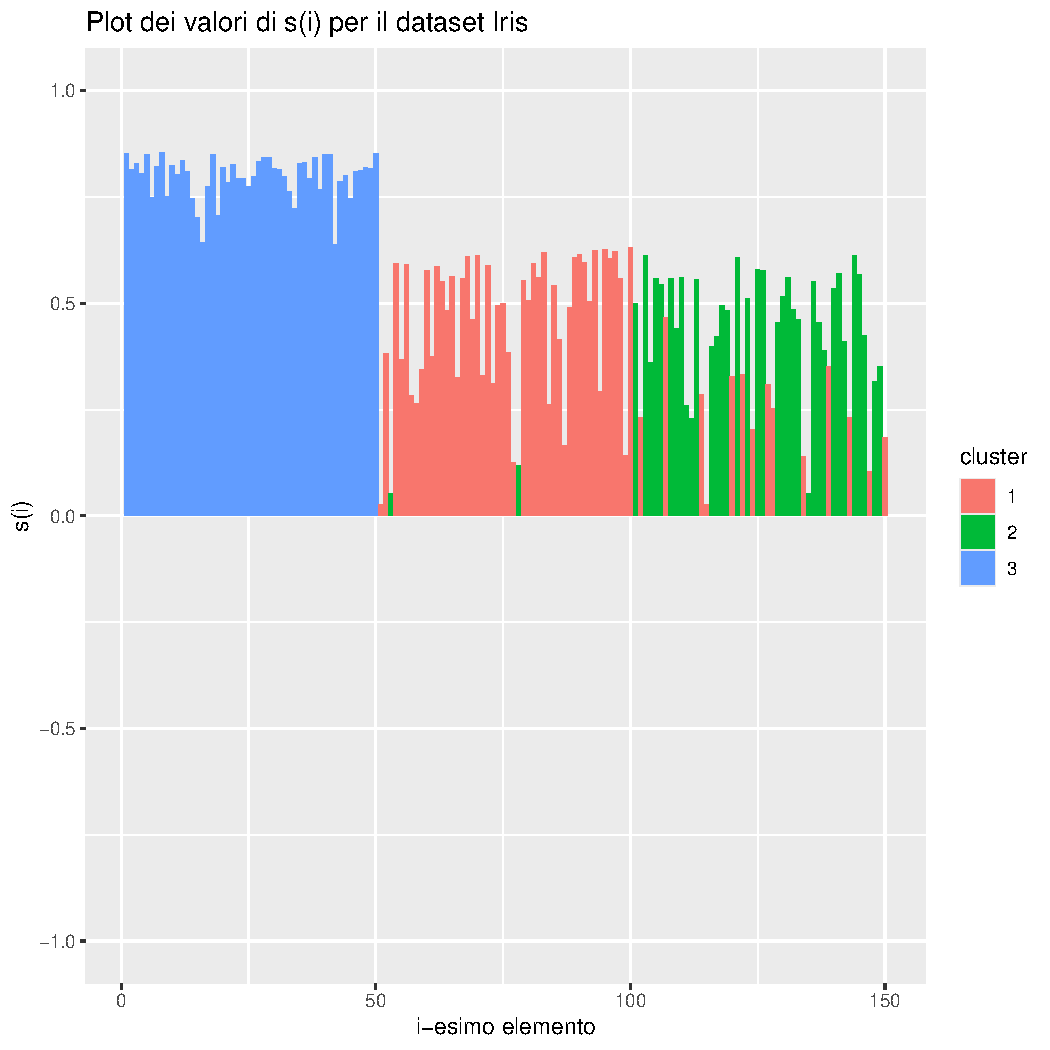
\includegraphics[width = 0.75\textwidth]{doc/si.pdf}
				\caption{Silhouette plot per il dataset \texttt{iris}, ottenuto
				dopo aver applicato K-Means con $K = 3$. Per ciascun elemento
				$i$ é riportato il valore di $s(i)$ ed il cluster a cui $i$
				é stato assegnato.}
				\label{fig:si}
			\end{figure}

			In generale, l'operato di un algoritmo di clustering può
			considerarsi ottimale se il valore si $s(i)$ tende ad essere
			molto alto per tutti gli elementi del dataset. A tale scopo,
			è possibile calcolare la Silhouette media per un certo cluster
			$C$ come la media tutti gli $s(i)$ per ciascun elemento $i$
			che appartiene a $C$. Se tale valore medio è alto, il cluster
			nel suo complesso è ben formato.

			Se si ha invece interesse a sapere qual'è il numero ottimale
			di cluster, è possibile considerare la Silhouette media
			complessiva come la media di tutti gli $s(i)$ per ogni
			elemento dell'intero dataset. Piú il valore della Silhouette
			media complessiva si avvicina ad $1$, piú il clustering
			interpreta correttamente la natura del dataset.

			\begin{figure}[H]
				\centering
				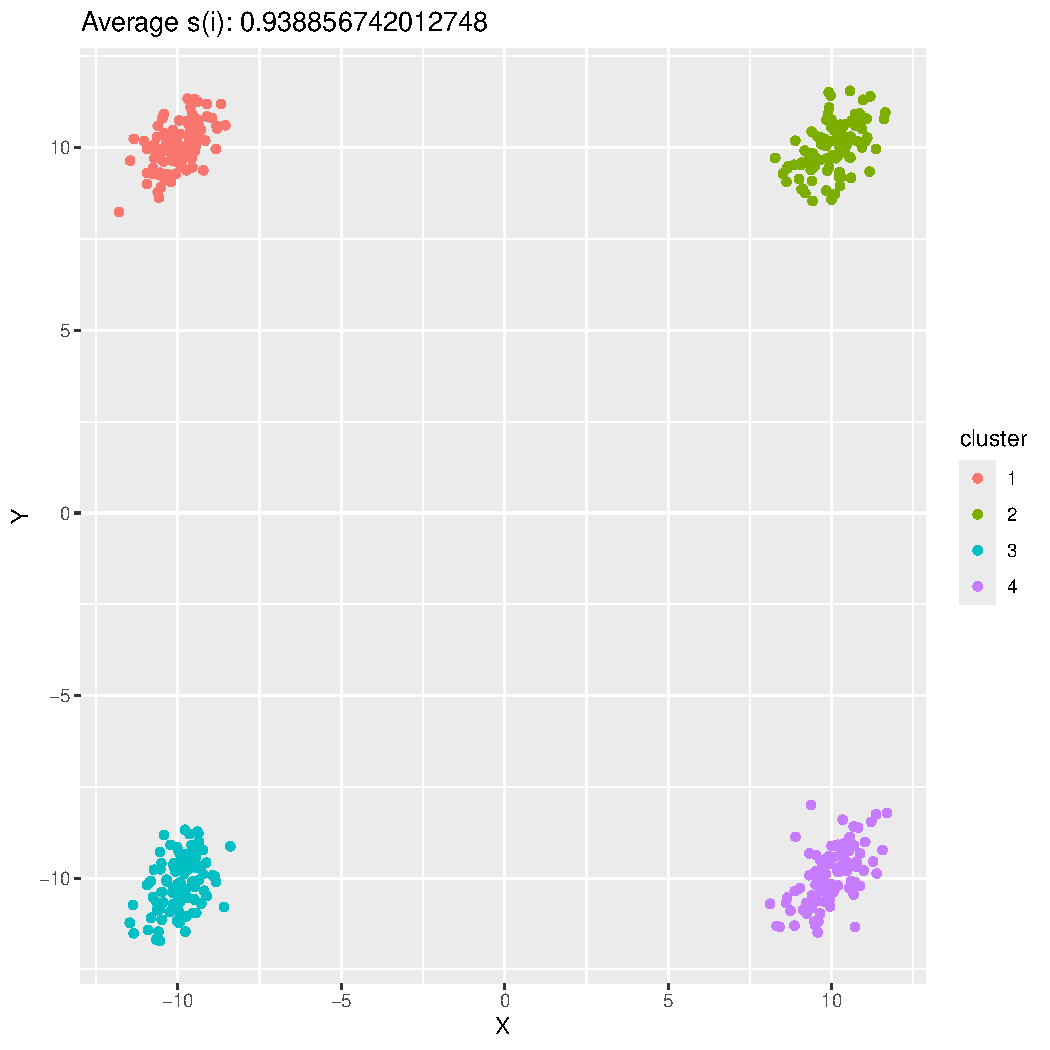
\includegraphics[width = 0.7\textwidth]{doc/clusters-4.pdf}
				\caption{Clustering indotto da K-Means con $K = 4$ su un
				dataset costituito da punti di normali bivariate, dove
				il numero di cluster rispecchia la naturale struttura
				del dataset. Si noti il valore della Silhouette media
				complessiva molto alto.}
				\label{fig:k4}
			\end{figure}

			Tutte le considerazioni fatte per i singoli valori di $s(i)$
			si estendono in maniera naturale alla Silhouette media
			complessiva. Si supponga ad esempio che un dataset abbia
			delle aree molto dense separate da aree ampie vuote. Operando
			un clustering in cui il numero di cluster è più basso del numero
			"naturale" di cluster, delle aree molto distanti tra loro vengono
			inglobate in un cluster unico nonostante vi siano considerevoli
			distanze nel mezzo. Silhouette può evidenziare questa situazione
			perché il valore di $a(i)$ tende ad essere molto alto, essendo
			i membri del dataset molto distanti dai loro centroidi. Di
			conseguenza, la Silhouette media complessiva sará bassa.

			\begin{figure}[H]
				\centering
				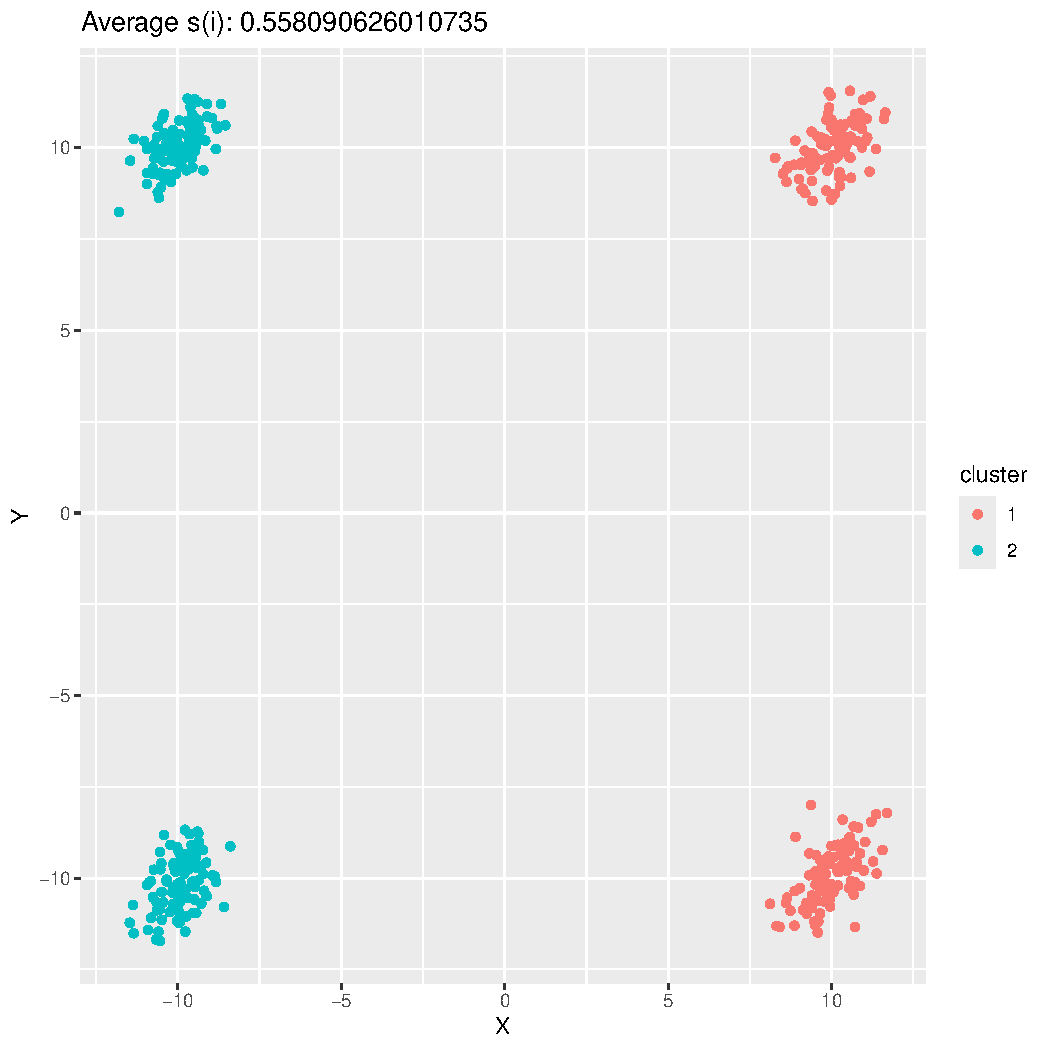
\includegraphics[width = 0.7\textwidth]{doc/clusters-2.pdf}
				\caption{Clustering indotto da K-Means con $K = 2$ su un
				dataset costituito da punti di normali bivariate, dove
				il numero di cluster é inferiore del numero di cluster
				naturali. Si noti il valore della Silhouette media
				complessiva basso.}
				\label{fig:k2}
			\end{figure}

			Si supponga invece di operare un clustering in cui il numero
			di cluster è più alto del numero "naturale" di cluster. In tale
			situazione, anche aree dense vengono spezzate in cluster diversi.
			Silhouette può evidenziare questa situazione perché il valore di
			$b(i)$ tende ad essere molto basso, dato che elementi molto vicini
			vengono separati forzosamente. Anche in questo caso, la Silhouette
			media complessiva sará bassa.

			\begin{figure}[H]
				\centering
				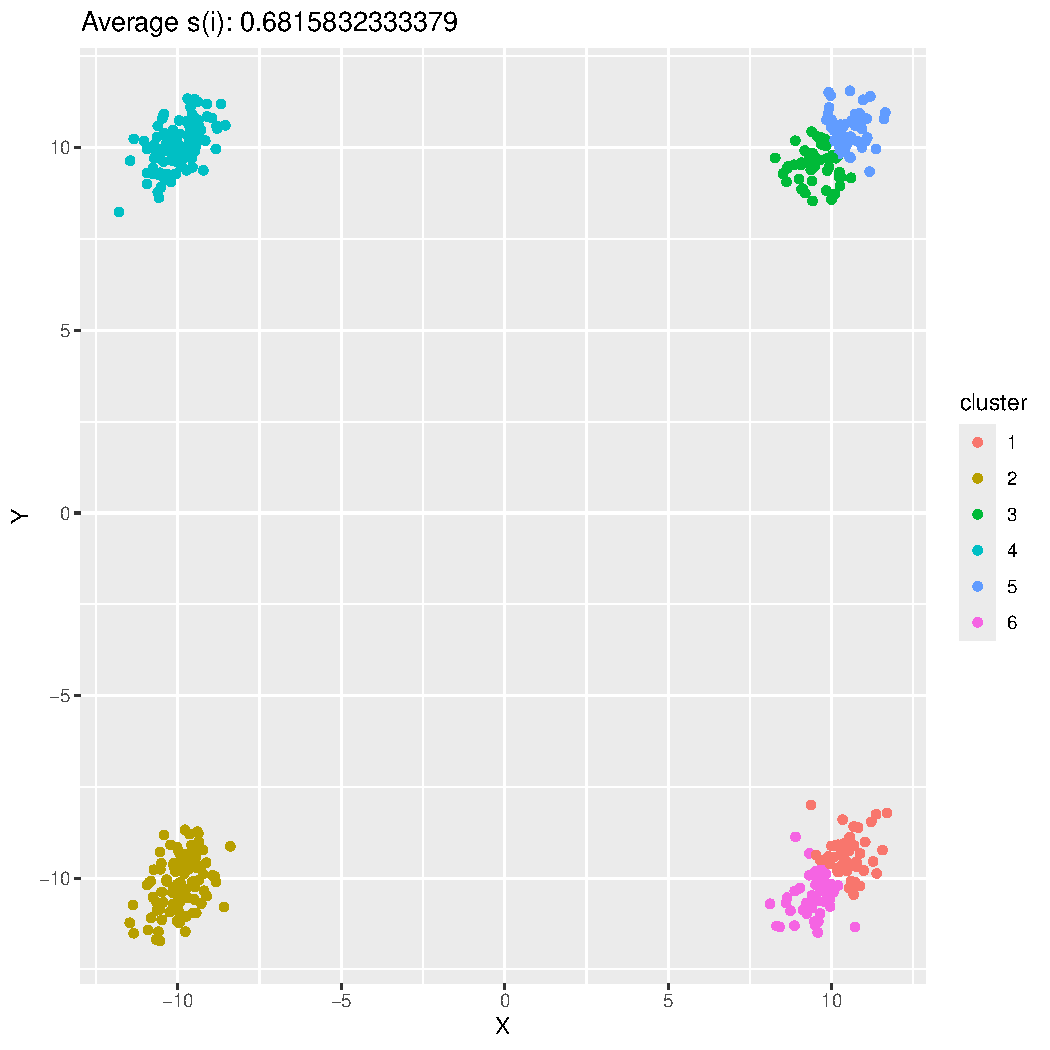
\includegraphics[width = 0.7\textwidth]{doc/clusters-6.pdf}
				\caption{Clustering indotto da K-Means con $K = 6$ su un
				dataset costituito da punti di normali bivariate, dove
				il numero di cluster é superiore al numero di cluster
				naturali. Si noti il valore della Silhouette media
				complessiva basso.}
				\label{fig:k6}
			\end{figure}

			Si noti come un valore della Silhouette media complessiva
			pari a $0$ non significa necessariamente che il clustering
			non sia andato a buon fine. Può infatti anche indicare che
			effettivamente il dataset non ha alcuna struttura di clustering
			naturale, e che quindi l'algoritmo di clustering ha comunque
			fornito un risultato corretto, dato che effettivamente qualsiasi
			risultato vale l'altro.

		\section{Test sanity check e matrice binaria}

			Il linguaggio \texttt{R} offre diverse implementazioni del
			calcolo della Silhouette. A differenza di altri linguaggi come
			Python, dove esiste un "consensus" (ufficiale o ufficioso) riguardo
			a quali siano i pacchetti da utilizzare per un determinato scopo,
			su \texttt{R} questo talvolta manca. Pertanto, prima di mettere
			Silhouette sotto analisi, è necessario scegliere un pacchetto fra
			quelli disponibili.

			Ho cercato quante più implementazioni di Silhouette possibili
			utilizzando il sito \texttt{https://rdrr.io} e scegliendo
			solamente quelli provenienti dal repository CRAN, di modo da
			avere la certezza di reperire solamente pacchetti di qualitá.
			In particolare, ho scelto \texttt{cluster}, \texttt{drclust},
			\texttt{tidyclust} e \texttt{Kira}. Pacchetti noti come
			\texttt{fpc}, che pure implementano Silhouette, li ho esclusi
			a priori perché non aggiornati da tempo.

			Oltre a questi, come controprova ho utilizzato l'implementazione
			della Silhouette presente nel pacchetto \texttt{scikit-learn} per
			\texttt{Python}. Questo è stato fatto attraverso il pacchetto
			\texttt{reticulate}, che permette di chiamare funzioni \texttt{Python}
			all'interno di codice \texttt{R}. Essendo \texttt{scikit-learn} 
			considerata una implementazione fidata, é possibile usarla come
			riferimento per fare dei confronti.

			Per comparare le performance delle diverse implementazioni di
			Silhouette ho eseguito due test, uno chiamato "sanity check" ed
			uno chiamato "matrice binaria".

			Il test sanity check prevede di applicare K-Means con $K = 2$
			sui dataset \texttt{sc\_dataset\_good} e \texttt{sc\_dataset\_bad}
			e calcolare la Silhouette media complessiva per entrambi. L'idea
			é che una implementazione corretta di Silhouette fornisca un
			valore molto alto per la Silhouette media complessiva rispetto
			al primo dataset, dove il numero di cluster scelto rispecchia
			perfettamente la struttura del dataset, ed un valore molto basso
			per il secondo, in cui i dati non hanno alcuna struttura.

			Il test matrice binaria prevede invece di generare una matrice
			di dimensione $20 \times 10$, costituita per metà da $0$ e per
			metà da $1$. Su tale matrice viene applicato K-Means con $K = 2$
			e si calcola la Silhouette media complessiva del risultato.
			Dopodiché, una qualsiasi delle righe viene sostituita con un
			valore scelto casualmente nell'intervallo $(0, 1)$ e si
			ripete il procedimento fino a quando tutte le righe hanno
			subito esattamente una sostituzione.

			I $2n$ valori della Silhouette media complessiva così trovati
			sono poi riportati in un plot; l'idea è che tali valori debbano
			essere alti nelle prime istanze del test quando gli $0$ e gli
			$1$ sono ben separati e, mano a mano che nel dataset vengono
			introdotti valori casuali, si abbassino sempre piú. Pur
			ammettendo delle flutturazioni, ci si aspetta che tali
			valori si distribuiscano linearmente.

	\chapter{Risultati ottenuti}

		\section{Risultati dei test sanity check su pacchetti R}

			Il risultati del test sanity check sono riportati nei plot
			seguenti. Per ciascun pacchetto sono riportati sia i valori
			della Silhouette media complessiva, sia il tempo di esecuzione
			necessario. Il colore degli elementi rappresenta il cluster
			nel quale è stato assegnato. Per ciascun pacchetto il test
			è stato ripetuto due volte: una volta usando \texttt{sc\_dataset\_good}
			ed una volta usando \texttt{sc\_dataset\_bad}.

			\begin{figure}[H]
				\centering
				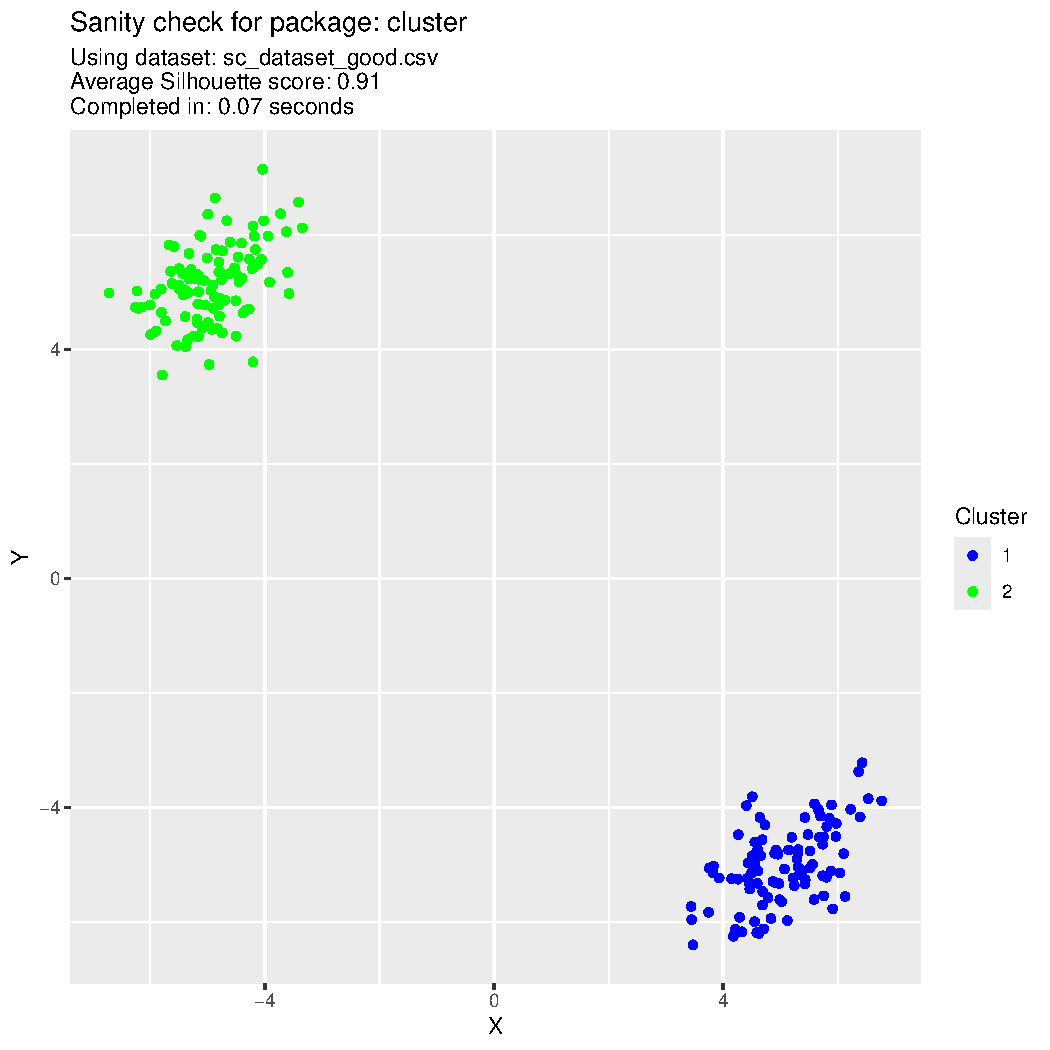
\includegraphics[width = 0.65\textwidth, page = 1]{results/results_CLUSTER.pdf}
				\caption{Risultato del test sanity check per il pacchetto \texttt{cluster}, usando \texttt{sc\_dataset\_good} come dataset.}
				\label{fig:clustergood}
			\end{figure}

			\begin{figure}[H]
				\centering
				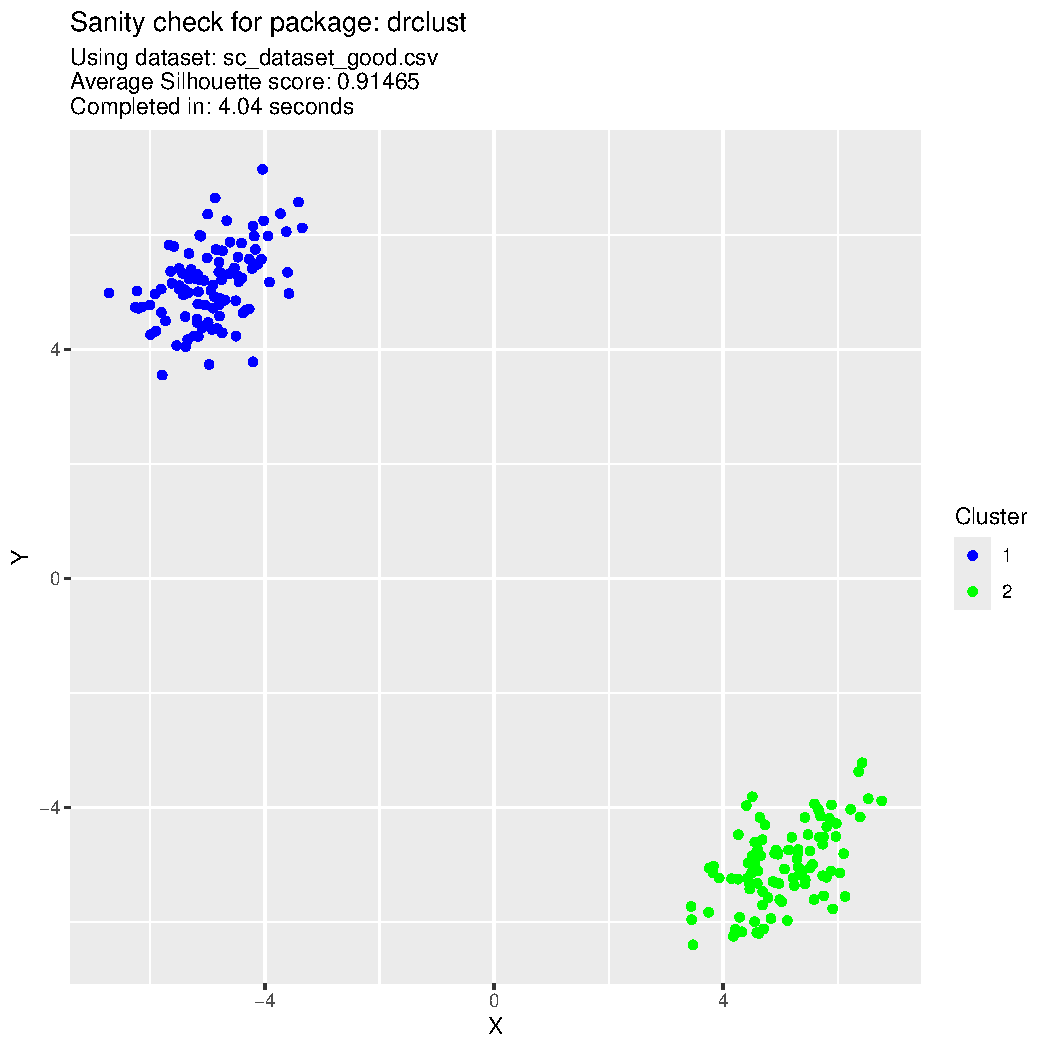
\includegraphics[width = 0.65\textwidth, page = 1]{results/results_DRCLUST.pdf}
				\caption{Risultato del test sanity check per il pacchetto \texttt{drclust}, usando \texttt{sc\_dataset\_good} come dataset.}
				\label{fig:drclustgood}
			\end{figure}

			\begin{figure}[H]
				\centering
				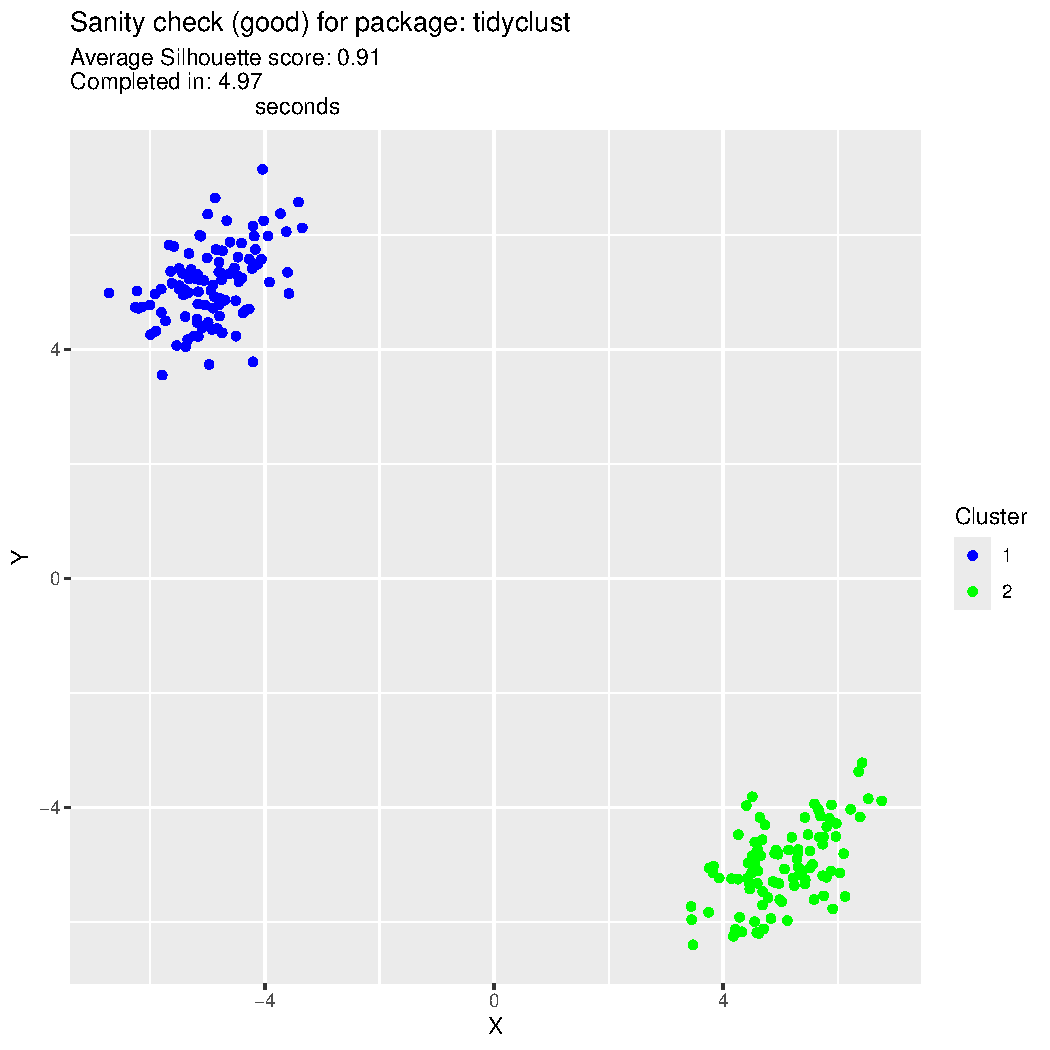
\includegraphics[width = 0.65\textwidth, page = 1]{results/results_TIDYCLUST.pdf}
				\caption{Risultato del test sanity check per il pacchetto \texttt{tidyclust}, usando \texttt{sc\_dataset\_good} come dataset.}
				\label{fig:tidyclustgood}
			\end{figure}

			\begin{figure}[H]
				\centering
				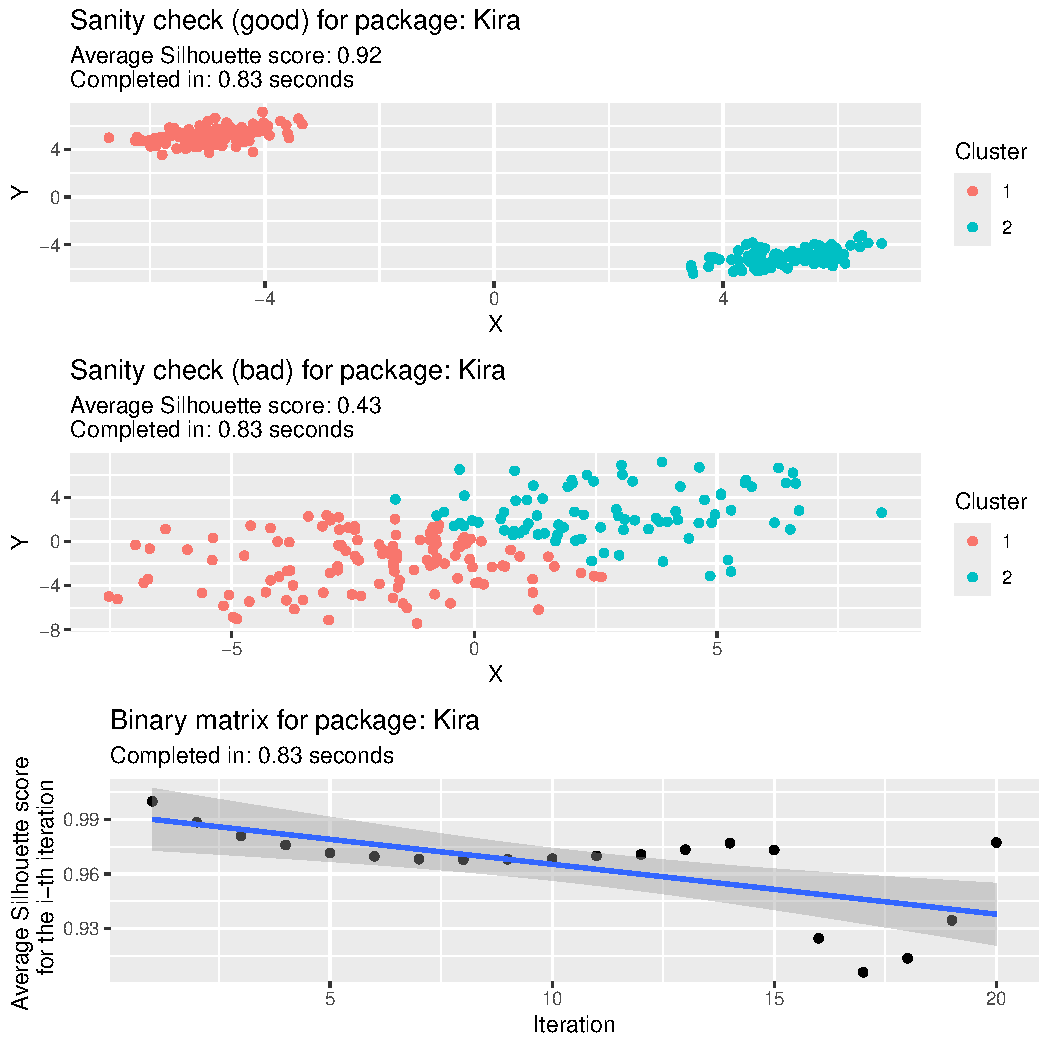
\includegraphics[width = 0.65\textwidth, page = 1]{results/results_KIRA.pdf}
				\caption{Risultato del test sanity check per il pacchetto \texttt{kira}, usando \texttt{sc\_dataset\_good} come dataset.}
				\label{fig:kiragood}
			\end{figure}

			\begin{figure}[H]
				\centering
				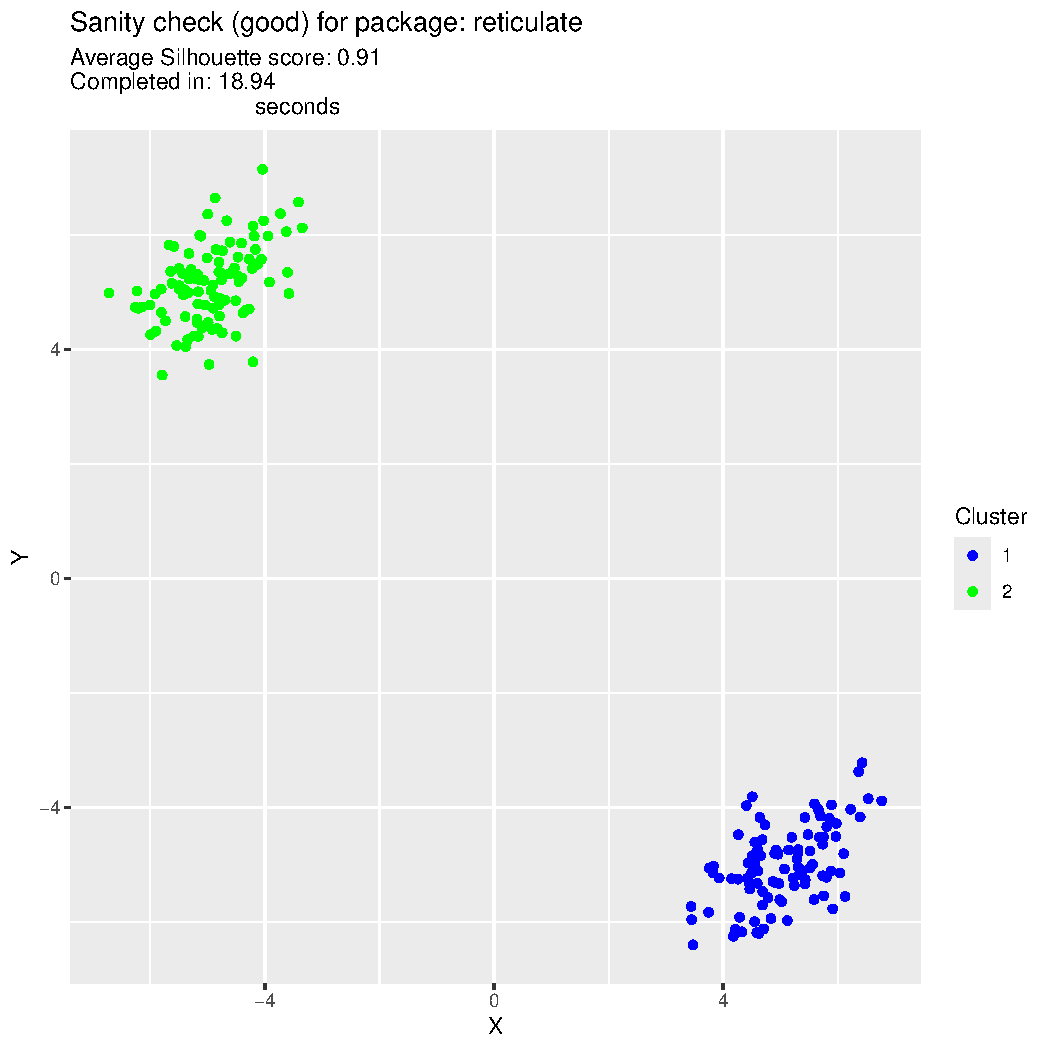
\includegraphics[width = 0.65\textwidth, page = 1]{results/results_RETICULATE.pdf}
				\caption{Risultato del test sanity check per il pacchetto \texttt{scikit-learn} tramite \texttt{reticulate}, usando \texttt{sc\_dataset\_good} come dataset.}
				\label{fig:reticulategood}
			\end{figure}

			\begin{figure}[H]
				\centering
				\includegraphics[width = 0.65\textwidth, page = 2]{results/results_CLUSTER.pdf}
				\caption{Risultato del test sanity check per il pacchetto \texttt{cluster}, usando \texttt{sc\_dataset\_bad} come dataset.}
				\label{fig:clusterbad}
			\end{figure}

			\begin{figure}[H]
				\centering
				\includegraphics[width = 0.65\textwidth, page = 2]{results/results_DRCLUST.pdf}
				\caption{Risultato del test sanity check per il pacchetto \texttt{drclust}, usando \texttt{sc\_dataset\_bad} come dataset.}
				\label{fig:drclustbad}
			\end{figure}

			\begin{figure}[H]
				\centering
				\includegraphics[width = 0.65\textwidth, page = 2]{results/results_TIDYCLUST.pdf}
				\caption{Risultato del test sanity check per il pacchetto \texttt{tidyclust}, usando \texttt{sc\_dataset\_bad} come dataset.}
				\label{fig:tidyclustbad}
			\end{figure}

			\begin{figure}[H]
				\centering
				\includegraphics[width = 0.65\textwidth, page = 2]{results/results_KIRA.pdf}
				\caption{Risultato del test sanity check per il pacchetto \texttt{kira}, usando \texttt{sc\_dataset\_bad} come dataset.}
				\label{fig:kirabad}
			\end{figure}
			
			\begin{figure}[H]
				\centering
				\includegraphics[width = 0.65\textwidth, page = 2]{results/results_RETICULATE.pdf}
				\caption{Risultato del test sanity check per il pacchetto \texttt{scikit-learn} tramite \texttt{reticulate}, usando \texttt{sc\_dataset\_bad} come dataset.}
				\label{fig:reticulatebad}
			\end{figure}

		\section{Risultati dei test matrice binaria su pacchetti R}

			I risultati per il test matrice binaria sono riportati nei plot
			seguenti. Per ciascun dataset, sono riportati i valori della
			Silhouette media complessiva per ciascuna delle 20 iterazioni
			dell'algoritmo. Sull'asse delle ascisse è riportato il numero
			delle iterazioni, mentre su quello delle ordinate il valore
			della Silhouette media complessiva. Essendo Silhouette un valore
			compreso fra $-1$ e $1$, le ordinate sono normalizzate su tale
			intervallo. Sovrimposta a tale sequenza di punti figura la retta
			di regressione lineare.

			\begin{figure}[H]
				\centering
				\includegraphics[width = 0.65\textwidth, page = 3]{results/results_CLUSTER.pdf}
				\caption{Risultato del test matrice binaria per il pacchetto \texttt{cluster}.}
				\label{fig:clusterbm}
			\end{figure}

			\begin{figure}[H]
				\centering
				\includegraphics[width = 0.65\textwidth, page = 3]{results/results_DRCLUST.pdf}
				\caption{Risultato del test matrice binaria per il pacchetto \texttt{drclust}.}
				\label{fig:drclustbm}
			\end{figure}

			\begin{figure}[H]
				\centering
				\includegraphics[width = 0.65\textwidth, page = 3]{results/results_TIDYCLUST.pdf}
				\caption{Risultato del test matrice binaria per il pacchetto \texttt{tidyclust}.}
				\label{fig:tidyclustbm}
			\end{figure}

			\begin{figure}[H]
				\centering
				\includegraphics[width = 0.65\textwidth, page = 3]{results/results_KIRA.pdf}
				\caption{Risultato del test matrice binaria per il pacchetto \texttt{kira}.}
				\label{fig:kirabm}
			\end{figure}
			
			\begin{figure}[H]
				\centering
				\includegraphics[width = 0.65\textwidth, page = 3]{results/results_RETICULATE.pdf}
				\caption{Risultato del test matrice binaria per il pacchetto \texttt{scikit-learn} tramite \texttt{reticulate}.}
				\label{fig:reticulatebm}
			\end{figure}

		\section{Risultati delle applicazioni di algoritmi di clustering su EHR}

			I risultati dell'applicazione dei quattro algoritmi di clustering
			sui dataset EHR citati sono riportati di seguito. Ciascuna
			combinazione algoritmo/dataset è formata da due plot.

			Il primo plot è una o più linee spezzate dove ciascun punto ha per
			ascissa il valore di un certo parametro e per ordinata il valore
			della Silhouette media complessiva del clustering operato usando
			tale parametro. Nel caso in cui i parametri dell'algoritmo siano
			due, sono riportate più rette, e ciascuna retta rappresenta la
			scelta di uno dei due parametri.

			Il secondo plot è un grafico a barre dove ciascuna colonna
			rappresenta, in percentuale, il numero di elementi che l'algoritmo
			ha assegnato a tale cluster.

			\begin{figure}[H]
				\centering
				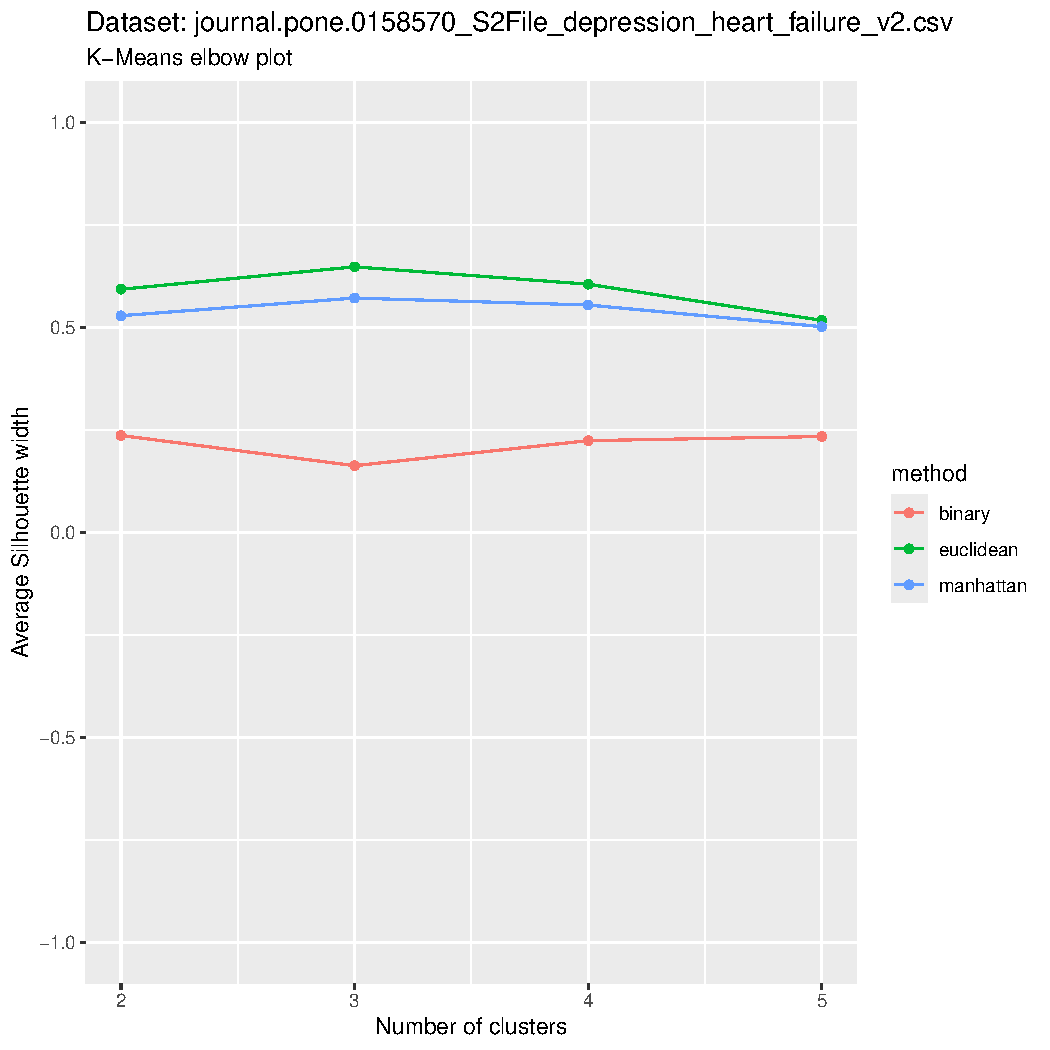
\includegraphics[width = 0.75\textwidth, height = 0.45\textheight, page = 1]{
					results/results_HeartFailure.csv.pdf
				}
				\includegraphics[width = 0.75\textwidth, height = 0.45\textheight, page = 2]{
					results/results_HeartFailure.csv.pdf
				}
				\caption{Risultati dell'algoritmo K-Means per il dataset
				\texttt{HeartFailure}}
				\label{fig:kmeans1}
			\end{figure}

			\begin{figure}[H]
				\centering
				\includegraphics[width = 0.75\textwidth, height = 0.45\textheight, page = 3]{
					results/results_HeartFailure.csv.pdf
				}
				\includegraphics[width = 0.75\textwidth, height = 0.45\textheight, page = 4]{
					results/results_HeartFailure.csv.pdf
				}
				\caption{Risultati dell'algoritmo K-Medians per il dataset
				\texttt{HeartFailure}}
				\label{fig:kmedians1}
			\end{figure}

			\begin{figure}[H]
				\centering
				\includegraphics[width = 0.75\textwidth, height = 0.45\textheight, page = 5]{
					results/results_HeartFailure.csv.pdf
				}
				\includegraphics[width = 0.75\textwidth, height = 0.45\textheight, page = 6]{
					results/results_HeartFailure.csv.pdf
				}
				\caption{Risultati dell'algoritmo DBSCAN per il dataset
				\texttt{HeartFailure}}
				\label{fig:dbscan1}
			\end{figure}

			\begin{figure}[H]
				\centering
				\includegraphics[width = 0.75\textwidth, height = 0.45\textheight, page = 7]{
					results/results_HeartFailure.csv.pdf
				}
				\includegraphics[width = 0.75\textwidth, height = 0.45\textheight, page = 8]{
					results/results_HeartFailure.csv.pdf
				}
				\caption{Risultati dell'algoritmo HDBSCAN per il dataset
				\texttt{HeartFailure}}
				\label{fig:hdbscan1}
			\end{figure}

			\begin{figure}[H]
				\centering
				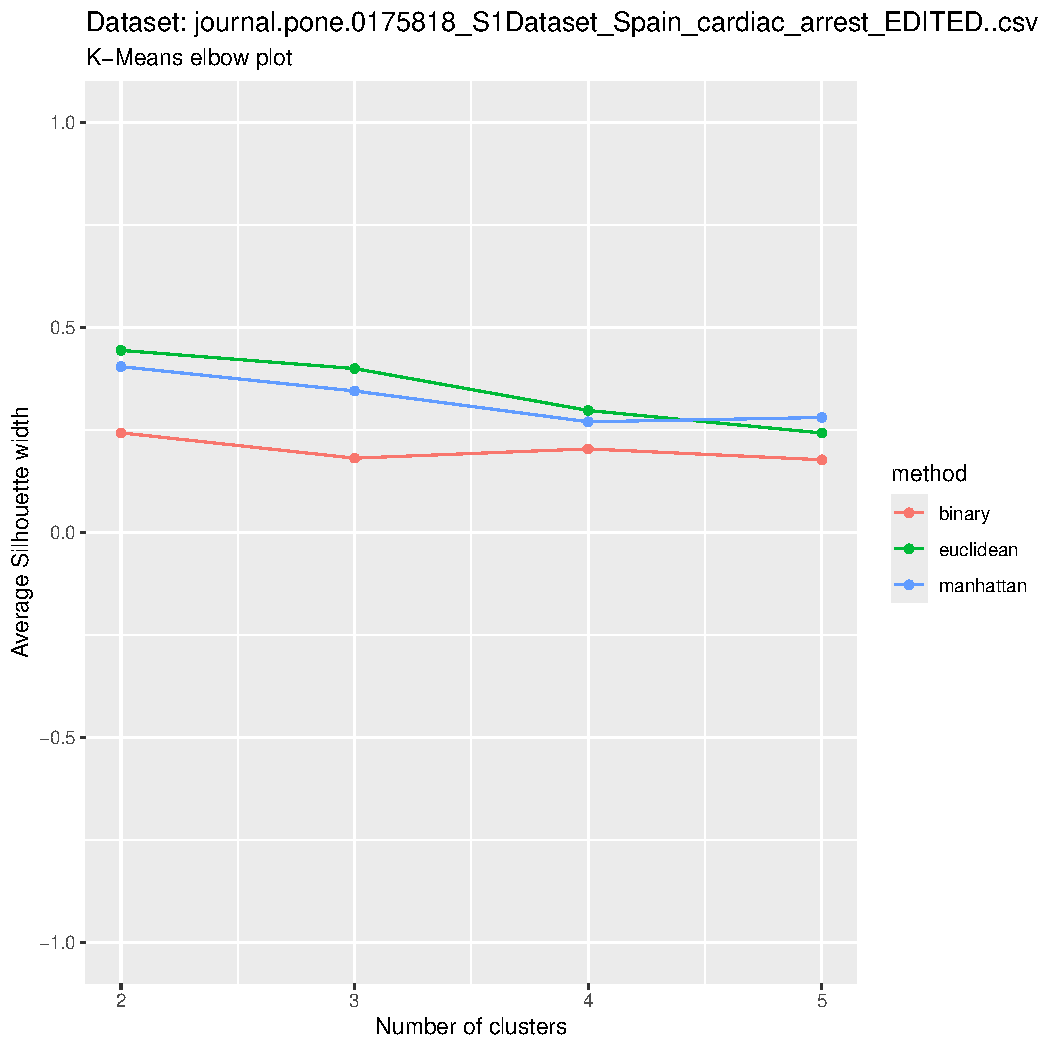
\includegraphics[width = 0.75\textwidth, height = 0.45\textheight, page = 1]{
					results/results_CardiacArrest.csv.pdf
				}
				\includegraphics[width = 0.75\textwidth, height = 0.45\textheight, page = 2]{
					results/results_CardiacArrest.csv.pdf
				}
				\caption{Risultati dell'algoritmo K-Means per il dataset
				\texttt{CardiacArrest}}
				\label{fig:kmeans2}
			\end{figure}

			\begin{figure}[H]
				\centering
				\includegraphics[width = 0.75\textwidth, height = 0.45\textheight, page = 3]{
					results/results_CardiacArrest.csv.pdf
				}
				\includegraphics[width = 0.75\textwidth, height = 0.45\textheight, page = 4]{
					results/results_CardiacArrest.csv.pdf
				}
				\caption{Risultati dell'algoritmo K-Medians per il dataset
				\texttt{CardiacArrest}}
				\label{fig:kmedians2}
			\end{figure}

			\begin{figure}[H]
				\centering
				\includegraphics[width = 0.75\textwidth, height = 0.45\textheight, page = 5]{
					results/results_CardiacArrest.csv.pdf
				}
				\includegraphics[width = 0.75\textwidth, height = 0.45\textheight, page = 6]{
					results/results_CardiacArrest.csv.pdf
				}
				\caption{Risultati dell'algoritmo DBSCAN per il dataset
				\texttt{CardiacArrest}}
				\label{fig:dbscan2}
			\end{figure}

			\begin{figure}[H]
				\centering
				\includegraphics[width = 0.75\textwidth, height = 0.45\textheight, page = 7]{
					results/results_CardiacArrest.csv.pdf
				}
				\includegraphics[width = 0.75\textwidth, height = 0.45\textheight, page = 8]{
					results/results_CardiacArrest.csv.pdf
				}
				\caption{Risultati dell'algoritmo HDBSCAN per il dataset
				\texttt{CardiacArrest}}
				\label{fig:hdbscan2}
			\end{figure}

			\begin{figure}[H]
				\centering
				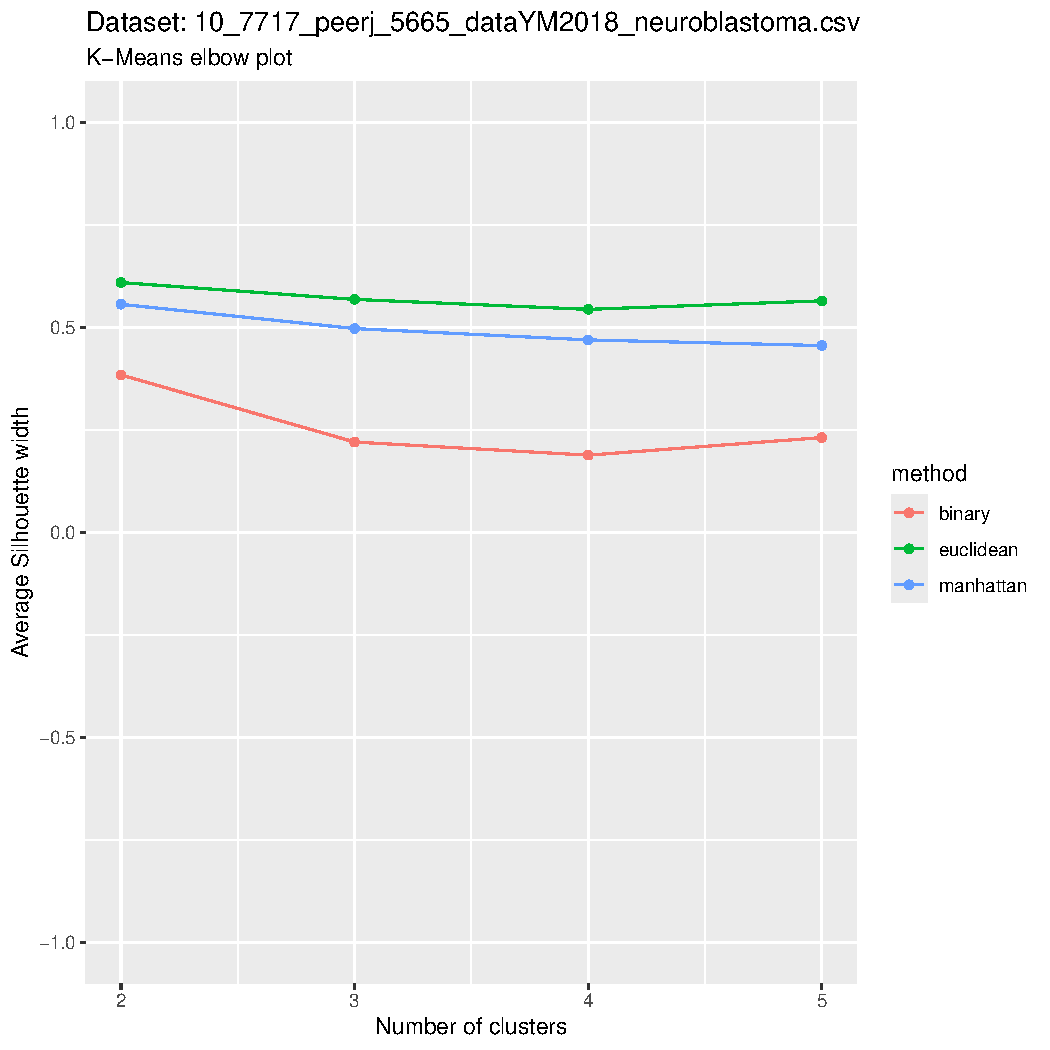
\includegraphics[width = 0.75\textwidth, height = 0.45\textheight, page = 1]{
					results/results_Neuroblastoma.csv.pdf
				}
				\includegraphics[width = 0.75\textwidth, height = 0.45\textheight, page = 2]{
					results/results_Neuroblastoma.csv.pdf
				}
				\caption{Risultati dell'algoritmo K-Means per il dataset
				\texttt{Neuroblastoma}}
				\label{fig:kmeans3}
			\end{figure}

			\begin{figure}[H]
				\centering
				\includegraphics[width = 0.75\textwidth, height = 0.45\textheight, page = 3]{
					results/results_Neuroblastoma.csv.pdf
				}
				\includegraphics[width = 0.75\textwidth, height = 0.45\textheight, page = 4]{
					results/results_Neuroblastoma.csv.pdf
				}
				\caption{Risultati dell'algoritmo K-Medians per il dataset
				\texttt{Neuroblastoma}}
				\label{fig:kmedians3}
			\end{figure}

			\begin{figure}[H]
				\centering
				\includegraphics[width = 0.75\textwidth, height = 0.45\textheight, page = 5]{
					results/results_Neuroblastoma.csv.pdf
				}
				\includegraphics[width = 0.75\textwidth, height = 0.45\textheight, page = 6]{
					results/results_Neuroblastoma.csv.pdf
				}
				\caption{Risultati dell'algoritmo DBSCAN per il dataset
				\texttt{Neuroblastoma}}
				\label{fig:dbscan3}
			\end{figure}

			\begin{figure}[H]
				\centering
				\includegraphics[width = 0.75\textwidth, height = 0.45\textheight, page = 7]{
					results/results_Neuroblastoma.csv.pdf
				}
				\includegraphics[width = 0.75\textwidth, height = 0.45\textheight, page = 8]{
					results/results_Neuroblastoma.csv.pdf
				}
				\caption{Risultati dell'algoritmo HDBSCAN per il dataset
				\texttt{Neuroblastoma}}
				\label{fig:hdbscan3}
			\end{figure}

			\begin{figure}[H]
				\centering
				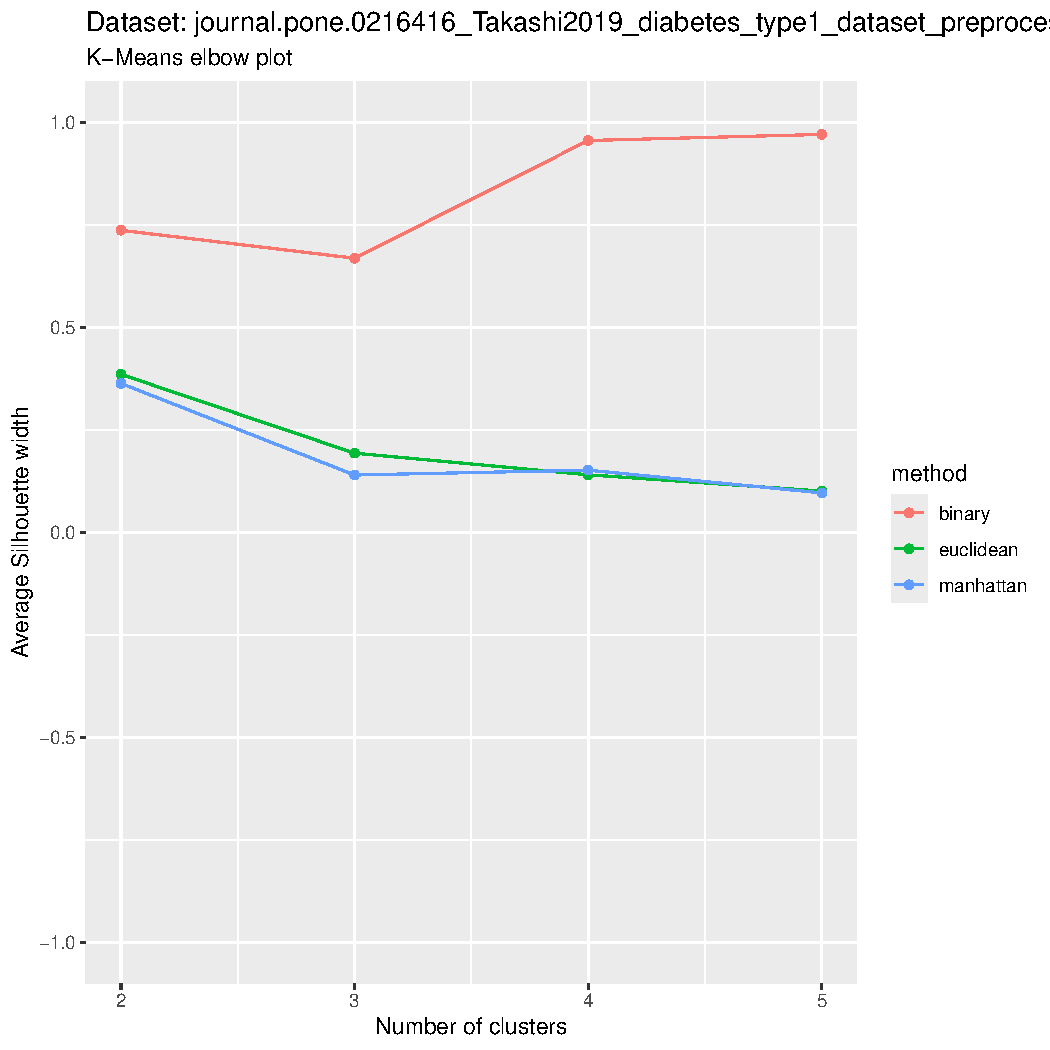
\includegraphics[width = 0.75\textwidth, height = 0.45\textheight, page = 1]{
					results/results_Diabetes.csv.pdf
				}
				\includegraphics[width = 0.75\textwidth, height = 0.45\textheight, page = 2]{
					results/results_Diabetes.csv.pdf
				}
				\caption{Risultati dell'algoritmo K-Means per il dataset
				\texttt{Diabetes}}
				\label{fig:kmeans4}
			\end{figure}

			\begin{figure}[H]
				\centering
				\includegraphics[width = 0.75\textwidth, height = 0.45\textheight, page = 3]{
					results/results_Diabetes.csv.pdf
				}
				\includegraphics[width = 0.75\textwidth, height = 0.45\textheight, page = 4]{
					results/results_Diabetes.csv.pdf
				}
				\caption{Risultati dell'algoritmo K-Medians per il dataset
				\texttt{Diabetes}}
				\label{fig:kmedians4}
			\end{figure}

			\begin{figure}[H]
				\centering
				\includegraphics[width = 0.75\textwidth, height = 0.45\textheight, page = 5]{
					results/results_Diabetes.csv.pdf
				}
				\includegraphics[width = 0.75\textwidth, height = 0.45\textheight, page = 6]{
					results/results_Diabetes.csv.pdf
				}
				\caption{Risultati dell'algoritmo DBSCAN per il dataset
				\texttt{Diabetes}}
				\label{fig:dbscan4}
			\end{figure}

			\begin{figure}[H]
				\centering
				\includegraphics[width = 0.75\textwidth, height = 0.45\textheight, page = 7]{
					results/results_Diabetes.csv.pdf
				}
				\includegraphics[width = 0.75\textwidth, height = 0.45\textheight, page = 8]{
					results/results_Diabetes.csv.pdf
				}
				\caption{Risultati dell'algoritmo HDBSCAN per il dataset
				\texttt{Diabetes}}
				\label{fig:hdbscan4}
			\end{figure}

			\begin{figure}[H]
				\centering
				\includegraphics[width = 0.75\textwidth, height = 0.45\textheight, page = 1]{
					results/results_Sepsis.csv.pdf
				}
				\includegraphics[width = 0.75\textwidth, height = 0.45\textheight, page = 2]{
					results/results_Sepsis.csv.pdf
				}
				\caption{Risultati dell'algoritmo K-Means per il dataset
				\texttt{Sepsis}}
				\label{fig:kmeans5}
			\end{figure}

			\begin{figure}[H]
				\centering
				\includegraphics[width = 0.75\textwidth, height = 0.45\textheight, page = 3]{
					results/results_Sepsis.csv.pdf
				}
				\includegraphics[width = 0.75\textwidth, height = 0.45\textheight, page = 4]{
					results/results_Sepsis.csv.pdf
				}
				\caption{Risultati dell'algoritmo K-Medians per il dataset
				\texttt{Sepsis}}
				\label{fig:kmedians5}
			\end{figure}

			\begin{figure}[H]
				\centering
				\includegraphics[width = 0.75\textwidth, height = 0.45\textheight, page = 5]{
					results/results_Sepsis.csv.pdf
				}
				\includegraphics[width = 0.75\textwidth, height = 0.45\textheight, page = 6]{
					results/results_Sepsis.csv.pdf
				}
				\caption{Risultati dell'algoritmo DBSCAN per il dataset
				\texttt{Sepsis}}
				\label{fig:dbscan5}
			\end{figure}

			\begin{figure}[H]
				\centering
				\includegraphics[width = 0.75\textwidth, height = 0.45\textheight, page = 7]{
					results/results_Sepsis.csv.pdf
				}
				\includegraphics[width = 0.75\textwidth, height = 0.45\textheight, page = 8]{
					results/results_Sepsis.csv.pdf
				}
				\caption{Risultati dell'algoritmo HDBSCAN per il dataset
				\texttt{Sepsis}}
				\label{fig:hdbscan5}
			\end{figure}

	\chapter{Discussione}

		\section{Classificazione dei pacchetti R}

			Sulla base dei test sanity check e matrice binaria é possibile
			trarre delle conclusioni in merito a quale pacchetto R che
			implementa Silhouette é da preferire.

			Il test sanity check non è stato particolarmente conclusivo,
			perché tutti e cinque i pacchetti hanno fornito valori molto
			simili (circa $0.9$ per \texttt{sc\_dataset\_good} e circa
			$0.4$ per \texttt{sc\_dataset\_bad}) e del tutto concordi con
			i risultati attesi. Questo non deve sorprendere, perché l'idea
			del test era di creare una situazione cosí estrema da evidenziare
			immediatamente la presenza di pacchetti problematici.

			Il test matrice binaria è stato invece più informativo, perché
			i valori restituiti avevano delle differenze evidenziabili. In
			particolare, \texttt{Kira} è stato il pacchetto con le performance
			peggiori, perché i valori della Silhouette media complessiva sono
			rimasti pressoché identici lungo tutte le iterazioni. I pacchetti
			\texttt{cluster}, \texttt{drclust} e \texttt{tidyclust} hanno
			invece avuto risultati molto simili. In particolare,
			\texttt{cluster} e \texttt{tidyclust} hanno avuto risultati
			perfettamente identici.

			Alla luce dei due test considerati, ho escluso immediatamente
			il pacchetto \texttt{Kira}, perché i risultati forniti dal test
			matrice binaria non sono affatto incoraggianti. Dato che i
			pacchetti \texttt{cluster} e \texttt{tidyclust} hanno fornito
			un risultato identico, fra i due ho preferito \texttt{cluster},
			perché ha un tempo di esecuzione più basso.

			Fra \texttt{cluster} e \texttt{drclust} ho preferito scegliere
			\texttt{cluster}. Questo sia perché il tempo di esecuzione è
			inferiore, sia perché il pacchetto \texttt{cluster} si trova
			spesso già incluso nelle installazioni di \texttt{R} (garanzia
			di affidabilità) sia perché è l'unico pacchetto il cui input
			non dipende dall'algoritmo usato. Infatti, \texttt{cluster}
			ha in input il risultato di un qualsiasi algoritmo di clustering
			ed una matrice delle distanze, mentre gli altri pacchetti
			richiedono in input espressamente il risultato di un algoritmo
			proveniente dal pacchetto da cui provengono, riducendone la
			portabilitá.

			Questo mi ha portato a scegliere \texttt{cluster} come
			pacchetto che implementasse Silhouette. Naturalmente, il
			pacchetto \texttt{scikit-learn} (attraverso \texttt{reticulate})
			non era preventivato che potesse essere scelto, dato che era
			stato incluso semplicemente come metro di paragone.

			A tal proposito, i plot successivi riportano il test matrice
			binaria applicato contemporaneamente sia a \texttt{cluster}
			che a \texttt{scikit-learn}, usando tre dimensioni diverse per
			la matrice, allo scopo di verificare di quanto i valori trovati
			si discostano. Come è possibile notare, la differenza fra i due
			è contenuta, e descresce con l'aumentare dell'aumentare delle
			dimensioni della matrice.

			\begin{figure}[H]
				\centering
				\includegraphics[width = 0.75\textwidth, page = 1]{results/Final_comparison.pdf}
				\caption{Test matrice binaria sia su \texttt{cluster} (pacchetto R) che su
				\texttt{scikit-learn} (pacchetto Python), usando una matrice $20 \times 10$.}
				\label{fig:cmp1}
			\end{figure}

			\begin{figure}[H]
				\centering
				\includegraphics[width = 0.75\textwidth, page = 2]{results/Final_comparison.pdf}
				\caption{Test matrice binaria sia su \texttt{cluster} (pacchetto R) che su
				\texttt{scikit-learn} (pacchetto Python), usando una matrice $100 \times 50$.}
				\label{fig:cmp2}
			\end{figure}

			\begin{figure}[H]
				\centering
				\includegraphics[width = 0.75\textwidth, page = 3]{results/Final_comparison.pdf}
				\caption{Test matrice binaria sia su \texttt{cluster} (pacchetto R) che su
				\texttt{scikit-learn} (pacchetto Python), usando una matrice $1000 \times 500$.}
				\label{fig:cmp3}
			\end{figure}

		\section{EHR}

			Come è possibile notare nei plot mostrati in precedenza,
			l'algoritmo scelto influenza notevolmente il numero di
			cluster che vengono individuati, pure se in ogni caso si
			tratta di iperparametri massimizzati usando Silhouette.
			Questo è in accordo con gli articoli citati. Di seguito
			sono riportate le performance degli algoritmi di clustering.

			\begin{figure}[H]
				\centering
				\includegraphics[width = 0.75\textwidth, height = 0.45\textheight, page = 9]{
					results/results_HeartFailure.csv.pdf
				}
				\includegraphics[width = 0.75\textwidth, height = 0.45\textheight, page = 10]{
					results/results_HeartFailure.csv.pdf
				}
				\caption{Riassunto dei risultati dei vari algoritmi per il dataset
				\texttt{HeartFailure}}
				\label{fig:comp1}
			\end{figure}

			\begin{figure}[H]
				\centering
				\includegraphics[width = 0.75\textwidth, height = 0.45\textheight, page = 9]{
					results/results_CardiacArrest.csv.pdf
				}
				\includegraphics[width = 0.75\textwidth, height = 0.45\textheight, page = 10]{
					results/results_CardiacArrest.csv.pdf
				}
				\caption{Riassunto dei risultati dei vari algoritmi per il dataset
				\texttt{CardiacArrest}}
				\label{fig:comp2}
			\end{figure}

			\begin{figure}[H]
				\centering
				\includegraphics[width = 0.75\textwidth, height = 0.45\textheight, page = 9]{
					results/results_Neuroblastoma.csv.pdf
				}
				\includegraphics[width = 0.75\textwidth, height = 0.45\textheight, page = 10]{
					results/results_Neuroblastoma.csv.pdf
				}
				\caption{Riassunto dei risultati dei vari algoritmi per il dataset
				\texttt{Neuroblastoma}}
				\label{fig:comp3}
			\end{figure}

			\begin{figure}[H]
				\centering
				\includegraphics[width = 0.75\textwidth, height = 0.45\textheight, page = 9]{
					results/results_Diabetes.csv.pdf
				}
				\includegraphics[width = 0.75\textwidth, height = 0.45\textheight, page = 10]{
					results/results_Diabetes.csv.pdf
				}
				\caption{Riassunto dei risultati dei vari algoritmi per il dataset
				\texttt{Diabetes}}
				\label{fig:comp4}
			\end{figure}

			\begin{figure}[H]
				\centering
				\includegraphics[width = 0.75\textwidth, height = 0.45\textheight, page = 9]{
					results/results_Sepsis.csv.pdf
				}
				\includegraphics[width = 0.75\textwidth, height = 0.45\textheight, page = 10]{
					results/results_Sepsis.csv.pdf
				}
				\caption{Riassunto dei risultati dei vari algoritmi per il dataset
				\texttt{Sepsis}}
				\label{fig:comp5}
			\end{figure}

			DBSCAN figura spesso come algoritmo dalle alte performance.
			Per tale motivo mi sono chiesto se fosse possibile testare
			le prestazioni di Silhouette su DBSCAN comparandolo con un
			metodo di ottimizzazione degli iperparametri alternativo, e
			vedere se i due risultati sono simili.

			Fissato MinPts come il doppio più uno delle dimensioni del dataset,
			il valore di $\epsilon$ può essere stimato costruendo un \textbf{KNN
			plot}: fissato $k = \textrm{MinPts} - 1$, lungo l'asse delle ascisse
			si riportano gli elementi ordinati in ordine crescente per distanza
			dal loro $k$-esimo vicino, mentre sull'asse delle ordinate la distanza
			stessa. In genere, una curva costruita sulla base di questi dati ha
			inizialmente un andamento stabile per poi avere una crescita rapida:
			il valore di $\epsilon$ è scelto il punto della curva in cui si ha
			tale variazione di pendenza.

			Come è possibile apprezzare nelle figure successive, i valori
			di $\epsilon$ così restituiti inducono un clustering che è molto
			simile a quello fornito utilizzando Silhouette. Questo indica che
			Silhouette è effettivamente in grado di restituire una combinazione
			ottimale di iperparametri.

			\begin{figure}[H]
				\centering
				\includegraphics[width = 0.75\textwidth, height = 0.45\textheight, page = 1]{
					doc/DBSCAN_optimal_MinPts.pdf
				}
				\includegraphics[width = 0.75\textwidth, height = 0.45\textheight, page = 1]{
					results/DBSCAN_visual_comparison.pdf
				}
				\caption{Risultati dell'algoritmo DBSCAN per il dataset
				\texttt{HeartFailure}, usando un KNN-plot per stimare $\epsilon$}
				\label{fig:dbscan-extra1}
			\end{figure}

			\begin{figure}[H]
				\centering
				\includegraphics[width = 0.75\textwidth, height = 0.45\textheight, page = 2]{
					doc/DBSCAN_optimal_MinPts.pdf
				}
				\includegraphics[width = 0.75\textwidth, height = 0.45\textheight, page = 2]{
					results/DBSCAN_visual_comparison.pdf
				}
				\caption{Risultati dell'algoritmo DBSCAN per il dataset
				\texttt{CardiacArrest}, usando un KNN-plot per stimare $\epsilon$}
				\label{fig:dbscan-extra2}
			\end{figure}

			\begin{figure}[H]
				\centering
				\includegraphics[width = 0.75\textwidth, height = 0.45\textheight, page = 3]{
					doc/DBSCAN_optimal_MinPts.pdf
				}
				\includegraphics[width = 0.75\textwidth, height = 0.45\textheight, page = 3]{
					results/DBSCAN_visual_comparison.pdf
				}
				\caption{Risultati dell'algoritmo DBSCAN per il dataset
				\texttt{Neuroblastoma}, usando un KNN-plot per stimare $\epsilon$}
				\label{fig:dbscan-extra3}
			\end{figure}

			\begin{figure}[H]
				\centering
				\includegraphics[width = 0.75\textwidth, height = 0.45\textheight, page = 4]{
					doc/DBSCAN_optimal_MinPts.pdf
				}
				\includegraphics[width = 0.75\textwidth, height = 0.45\textheight, page = 4]{
					results/DBSCAN_visual_comparison.pdf
				}
				\caption{Risultati dell'algoritmo DBSCAN per il dataset
				\texttt{Diabetes}, usando un KNN-plot per stimare $\epsilon$}
				\label{fig:dbscan-extra4}
			\end{figure}

			\begin{figure}[H]
				\centering
				\includegraphics[width = 0.75\textwidth, height = 0.45\textheight, page = 5]{
					doc/DBSCAN_optimal_MinPts.pdf
				}
				\includegraphics[width = 0.75\textwidth, height = 0.45\textheight, page = 5]{
					results/DBSCAN_visual_comparison.pdf
				}
				\caption{Risultati dell'algoritmo DBSCAN per il dataset
				\texttt{Sepsis}, usando un KNN-plot per stimare $\epsilon$}
				\label{fig:dbscan-extra5}
			\end{figure}

		\section{Oltre Silhouette?}

			A partire dall'idea di base di Silhouette, è possibile costruirne
			infinite varianti. Gli autori citano:

			\begin{itemize}
				\item
				Per determinare il miglior numero di cluster non è strettamente
				necessario utilizzare la Silhouette media complessiva. Sarebbe
				infatti possibile anche combinare gli $s(i)$ in modo diverso;
				\item
				La Silhouette media complessiva può essere essa stessa usata
				come funzione obiettivo da massimizzare direttamente all'interno
				di un algoritmo di clustering, anziché effettuare una valutazione
				a posteriori;
				\item
				Se l'algoritmo di clustering si basa sulla costruzione di centroidi
				o sulla elezione di rappresentanti, si potrebbe usare la distanza
				da tali centroidi o rappresentanti come grado di dissomiglianza
				anziché calcolare $a(i)$ o $D(i, C)$ per ogni $i$-esimo elemento,
				semplificando il procedimento. Naturalmente, questo approccio
				renderebbe Silhouette dipendente dal tipo di algoritmo usato. 
			\end{itemize}

			Tutte e tre le varianti sono toccate da articoli citati.

	\chapter{Conclusioni}

		Data la natura di questa tesi, é evidente come questo non possa
		essere altro che un lavoro esplorativo. Le idee qui presentate
		potrebbero essere estese in diversi modi, alcuni riportati di
		seguito.

		Innanzitutto, i test sono stati condotti usando esclusivamente EHR
		come dataset. Sebbene queste contengano moltissime informazioni, non
		sono una risorsa omnicomprensiva. Si potrebbe pertanto ripetere i
		test utilizzando anche o soltanto dataset di dati biomedici che
		contengono dati che le EHR ignorano, dando un quadro piú completo.

		Inoltre, gli algoritmi di clustering sono stati applicati su dataset
		dove parte degli elementi avevano uno o più attributi di valore
		ignoto. Non essendo possibile operare il clustering con dati dei
		quali non è noto il valore, l'approccio che ho utilizzato è
		semplicemente stato quello di eliminare ogni elemento che avesse
		almeno un dato mancante. Si potrebbe ripetere gli esperimenti
		adottando un approccio più conservativo, ad esempio sostituendo
		tali dati con valori di default ed osservare se si presentano
		differenze.

		Un'alternativa simile è quella di utilizzare tecniche in grado di
		predire i valori mancanti sulla base di quelli noti, ad esempio
		calcolando la media di tutti i valori noti per un certo attributo
		ed utilizzarla al posto dei valori mancanti.

		Infine, sarebbe interessante ripetere gli esperimenti operando
		\textbf{dimensionality reduction}, come ad esempio \textbf{principal
		component analysis} \cite{Hotelling1933AnalysisOA}, ovvero tecniche
		in grado di accorpare o di scartare del tutto gli attributi che non
		hanno particolare rilevanza nel risultato finale del clustering.
		Questo permetterebbe, ammesso di riuscire a ridurre il numero delle
		dimensioni fino a due o a tre, di poter visualizzare il risultato
		del clustering in uno scatter plot, a prescindere dal numero originale
		delle dimensioni.

	\chapter*{Disponibilitá del codice}

		Il codice per la generazione dei test e per l'applicazione degli
		algoritmi di clustering ai dataset EHR è liberamente disponibile.
		Il codice in questione puó essere reperito al seguente link:

		\texttt{https://github.com/Skimmeroni/Silhouette-Unimib-thesis}.

		Ho organizzato il codice seguendo le linee guida riportate in
		\cite{10.1371/journal.pcbi.1000424}. Ho anche tenuto un lab
		notebook per tenere traccia dei risultati mano mano che venivano
		generati, facendo riferimento a \cite{10.1371/journal.pcbi.1004385}.

	\printbibliography

\end{document}


\end{sile}
